\documentclass{template/openetcs_article}
% Use the option "nocc" if the document is not licensed under Creative Commons
%\documentclass[nocc]{template/openetcs_article}
\usepackage{lipsum,url}
\usepackage{supertabular}
\usepackage{multirow}
\usepackage{hhline}
\usepackage{textcomp} %added by Mairamou
\usepackage{float} %added by Mairamou
\usepackage{color, colortbl}
\definecolor{gray}{rgb}{0.8,0.8,0.8}
\usepackage[modulo]{lineno}
\graphicspath{{./template/}{.}{./images/}}
\begin{document}
\frontmatter
\project{openETCS}

%Please do not change anything above this line
%============================



% The document metadata is defined below

%assign a report number here
\reportnum{OETCS/WP3 D3.5.3 Trackside}

%define your workpackage here
\wp{Work-Package 3: ``Modeling" }

%set a title here
\title{Dynamic ETCS Track Model}

%set a subtitle here
\subtitle{Use Case: Amsterdam- Utrecht ETCS L2 Reference Line}

%set the date of the report here
\date{August 2015}


%document approval
%define the name and affiliation of the people involved in the documents approbation here
\creatorname{Jakob G\"artner}
\creatoraffil{LEA Railergy}

\techassessorname{Baseliyos Jacob}
\techassessoraffil{DB Netz AG}

\qualityassessorname{Marc Behrens}
\qualityassessoraffil{DLR}

\approvalname{Klaus-R\"udiger Hase}
\approvalaffil{DB Netz AG}


%define a list of authors and their affiliation here

\author{Mairamou Haman Adji}

\affiliation{LEA Railergy\\
  c/o LEA P\&W sarl\\
  BP14000 \\
  Yaound\'e,\\ R\'epublique du Cameroun\\}

%\author{Jakob G\"artner}

%\affiliation{LEA Railergy\\
%Am Mittleren Moos 48\\
%86167 Augsburg, Germany}




% define the coverart
\coverart[width=350pt]{openETCS_EUPL}

%define the type of report
\reporttype{Track Model User's Guide}


\begin{abstract}
%define an abstract here

openETCS provides a formalisation of a reference ETCS onboard unit, using model- based software design based on the Scade language.\newline
In order to complement this work with a dynamic simulation environment  a ETCS track model has been developed. In contrast to pure scenario- driven approach, this model is intended to provide a simulation of dynamic behaviour of the track based on active interaction between train and track. The model has been derived from actual engineering data and events that have been collected by a train passing this reference track.
This document provides an outline of the simulation concept, its implementation and is intended to serve as a quick reference guide to users and reviewers.\newline On purpose, it has been written in a semi- technical way in order to be understandable by a more general audience. However, some basic understanding of ETCS is helpful for the reception of this document.

\end{abstract}

%=============================
\maketitle

%Modification history
%if you do not need a modification history table for your document simply comment out the eight lines below
%=============================


\section*{Modification History}
\tablefirsthead{
\hline 
\rowcolor{gray} 
Version & Section & Modification / Description & Author \\\hline}
\begin{supertabular}{| m{1.2cm} | m{1.2cm} | m{6.6cm} | m{4cm} |}
 1.0 &  all & created document & Mairamou Haman Adji\\\hline
\end{supertabular}


\tableofcontents
\listoffiguresandtables
\newpage
%=============================

%Uncomment the next line if you need line numbers for traceability when the document is in review
%\linenumbers
%=============================


% The actual document starts below this line
%=============================

%Start here











\section{Proof of Concept based on User Stories}

One of the main objectives of the openETCS project is to prove the formalisation of the EVC by validating it against a reference track. The project has selected the ETCS Level 2 track between Utrecht and Amsterdam (The Netherlands) as the reference track of choice.\newline
openETCS is using the concept of \emph{user stories} to define meaningful use cases from the point of view of a railway operator. DB Netz AG as the project leader has defined the following scenarios in order to focus and drive the project's priorities:
\begin{itemize}
 \item{Use case 1: Start of Mission and connection to the RBC (Issue \#66)}
 \item{Use Case 2: Train is running after receiving a Movement Authority (MA); (Issue \#67)}
 \item{Use Case 3: ETCS Brake intervention (revocation of MA or not allowed speed); (Issue \#68)}
 \item{Use Case 4: Train is reading track information - Train is sending information to the track. (Issue \#69)}
 \item{Use Case 5: Awakeness of Train with Level NTC (Issue \#244)}
 \item{Use Case 6: SoM in Level NTC and Mode SN (Issue \#245)}
 \item{Use Case 7: Running in Level NTC and Mode SN (Issue \#246)}
 \item{Use Case 8: Change Level NTC and SN to Level 2 and Mode FS (Issue \#247)}
 \item{Use Case 9: Run in Level 2 and Mode FS after MA request (Issue \#248)}
 \item{Use Case 10: Change Level 2 Mode FS to Level NTC Mode SN (Issue \#249)}
 \item{Use Case 11: Run in Level NTC and Mode SN (Issue \#250)}
 \item{Use Case 12: End of Mission in Level NTC and Mode SN (Issue \#251)}
 \item{Use Case 13: Train stops before Signal Marker Board after revoked Movement Authority (MA); (Issue \#70)}
 \item{Use Case 14: Mode Change and communication with the RBC. (Issue \#71)}
 \item{Use Case 15: Route is cancelled from the end of route signal. (Issue \#72)}
 \item{Use Case 16: Behaviour of the OBU after a TRIP. (Issue \#73)}
\end{itemize}

\emph{(Non-exhaustive list: The authoritative definition of the User Stories can be found on\newline https://github.com/openETCS/modeling/issues\newline and can be identified by the issue number cited above, or by searching for the label "User Story")}

The Use Cases can be roughly classified as follows:
\begin{enumerate}
 \item Use cases that are directly derived from existing data taken from a test train passing the Amsterdam- Utrecht ETCS L2 line
 \item Use cases that are derived from test requirements for the Amsterdam- Utrecht and are based on synthetic data, created on purpose.
\end {enumerate}

Use case 7 (please see figure \ref{fig:us07}) is a typical use case that can be represented using the nominal behaviour taken from data recorded during a train passage.

\begin{figure}
  \centering
  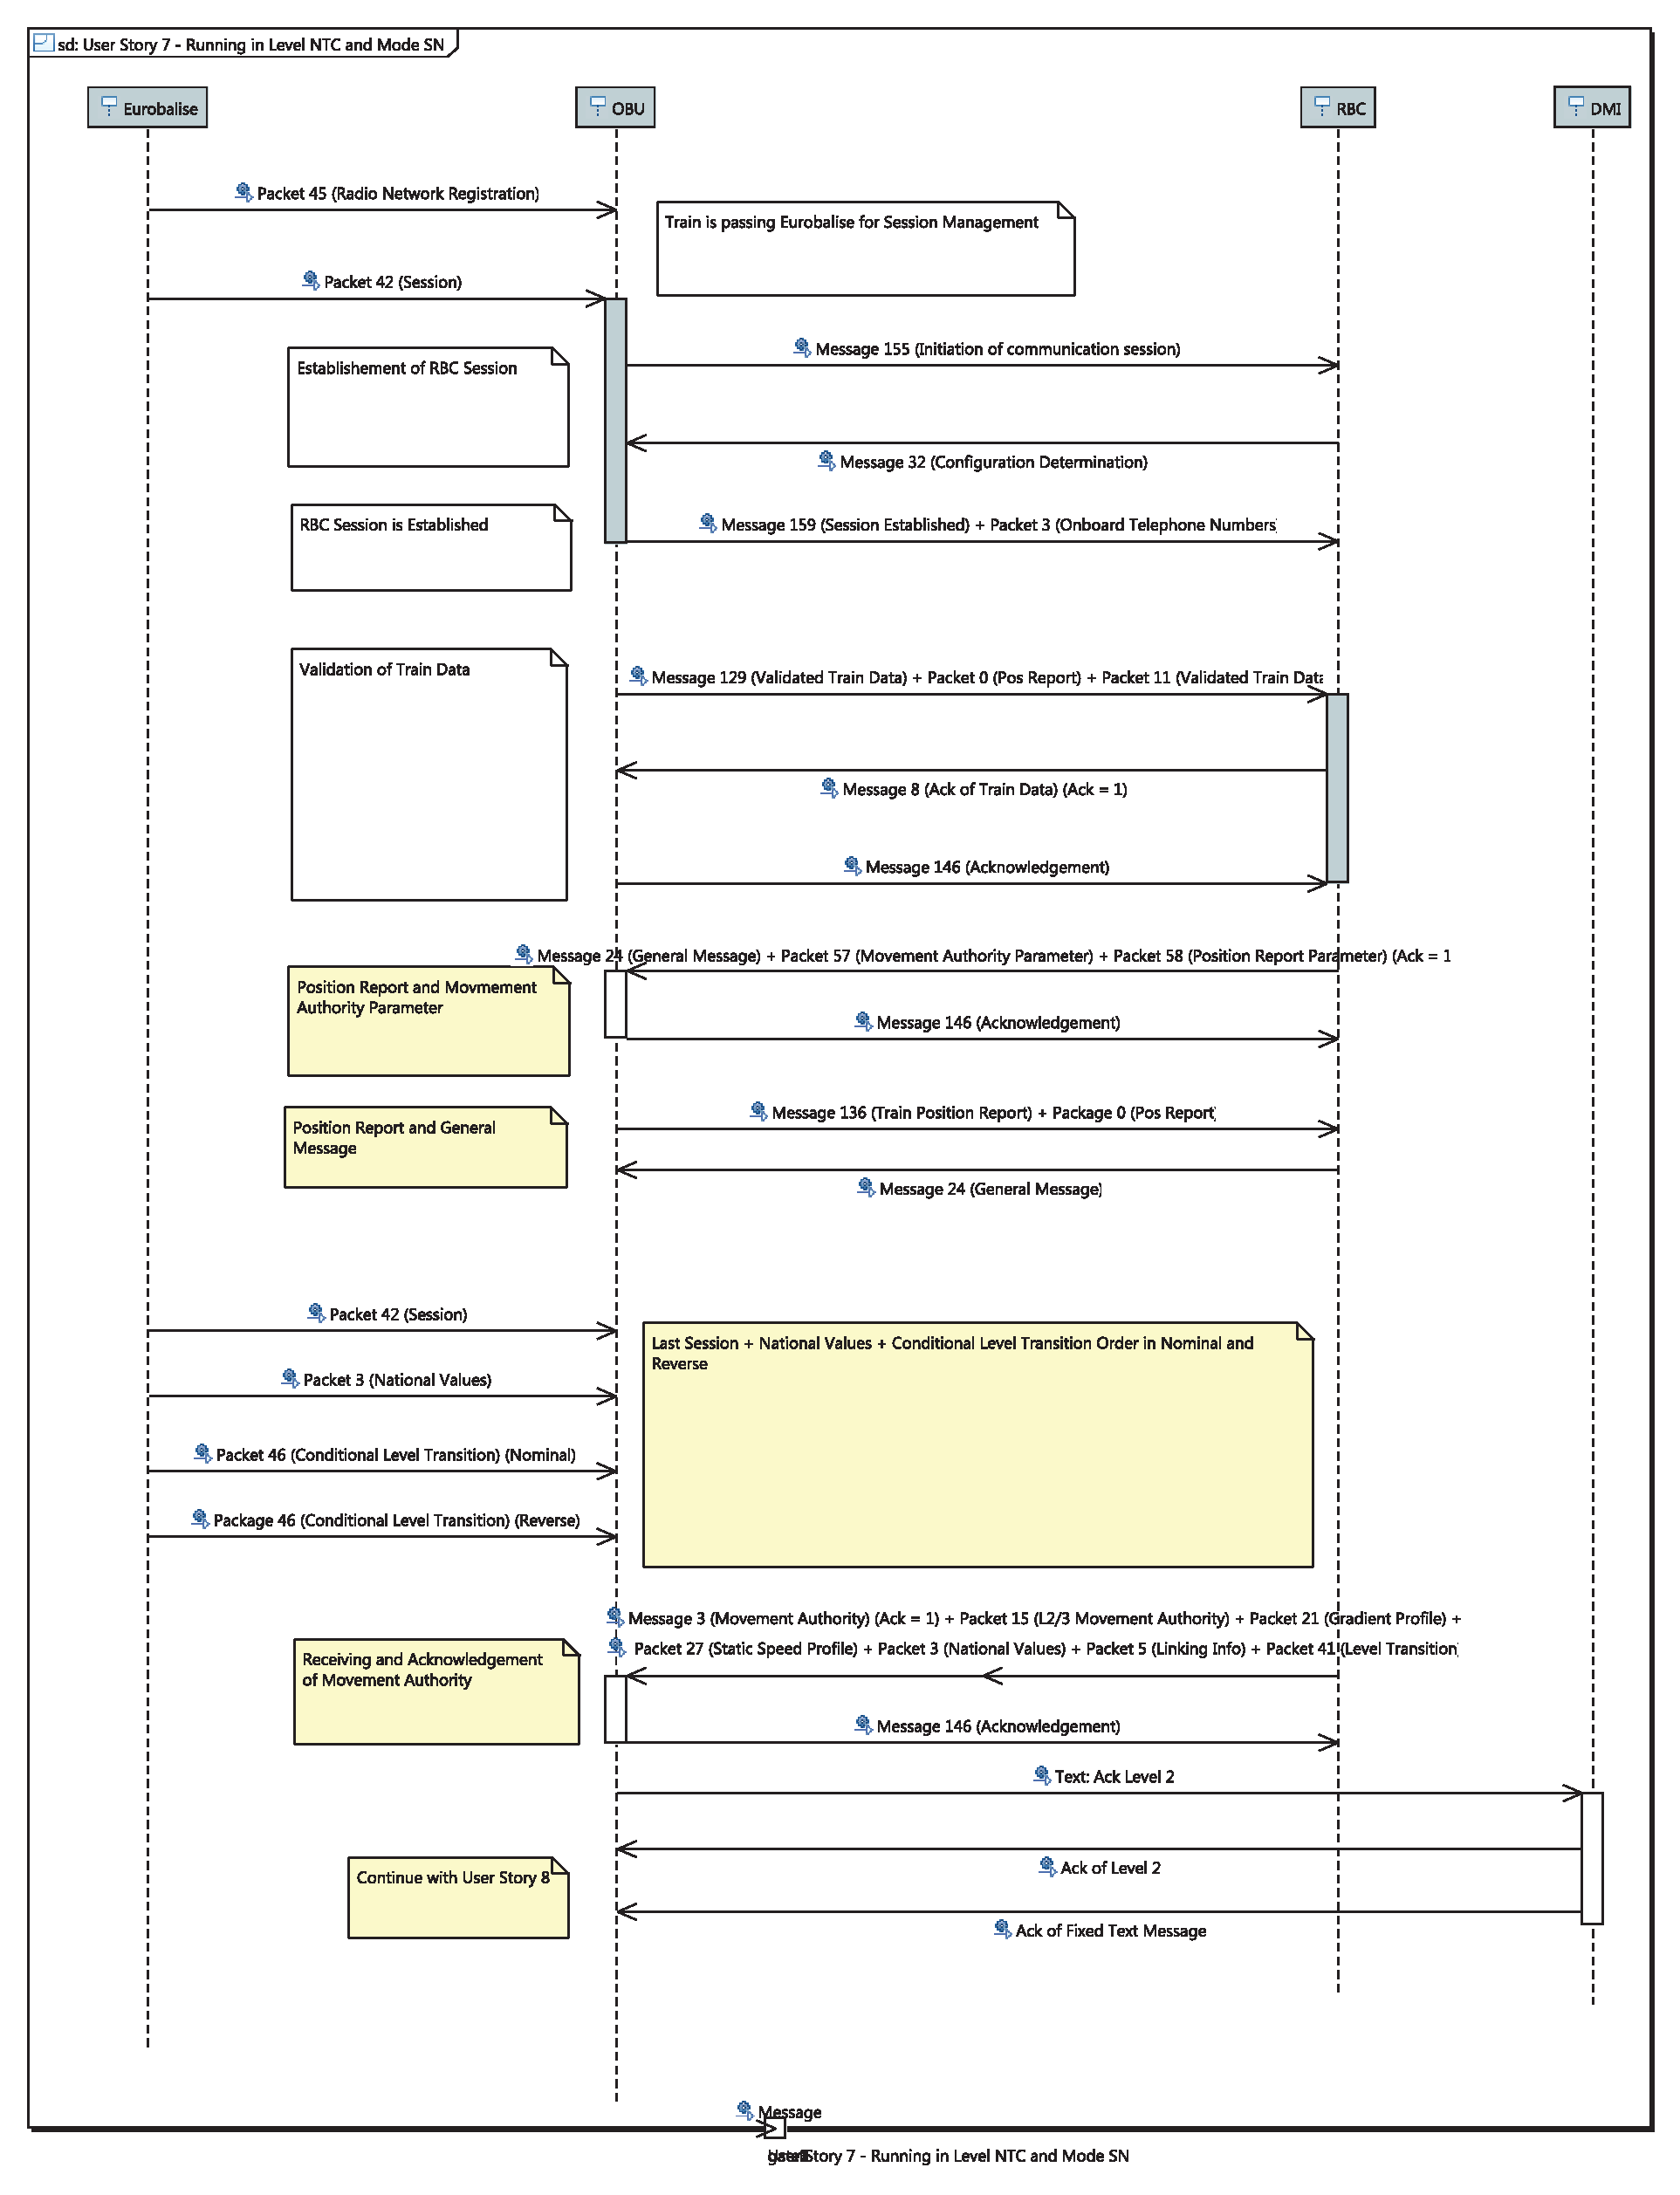
\includegraphics[width=6.5in]{images/UserStory7-2-sequence.eps}
  \caption{Example for a "nominal" user story: Sequence Diagram for Use Case 7}
  \label{fig:us07}
\end{figure}

Other use cases appear to be more complex: to reproduce them, we have to create a specific situation that may only be done at very high cost (by interrupting normal train operations for test rides) or by creating a specific simulation scenario. An example for such a scenario is Use Case 13. (see figure \ref{fig:d-us13})

\begin{figure}
  \centering
  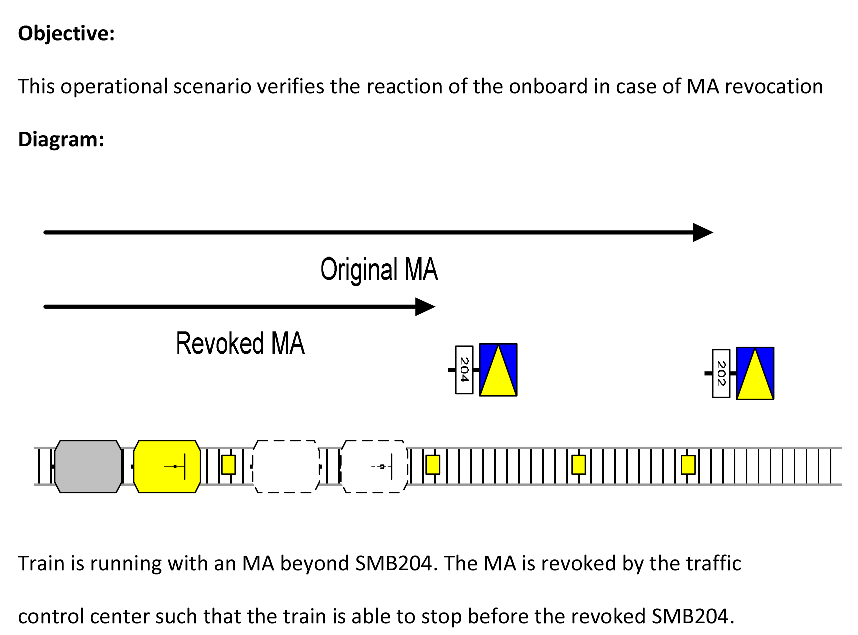
\includegraphics[width=5in]{images/DescrUserStory13.eps}
  \caption{Example for a "test case" user story: Description for Use Case 13}
  \label{fig:d-us13}
\end{figure}

%\begin{figure}
 % \centering
 % 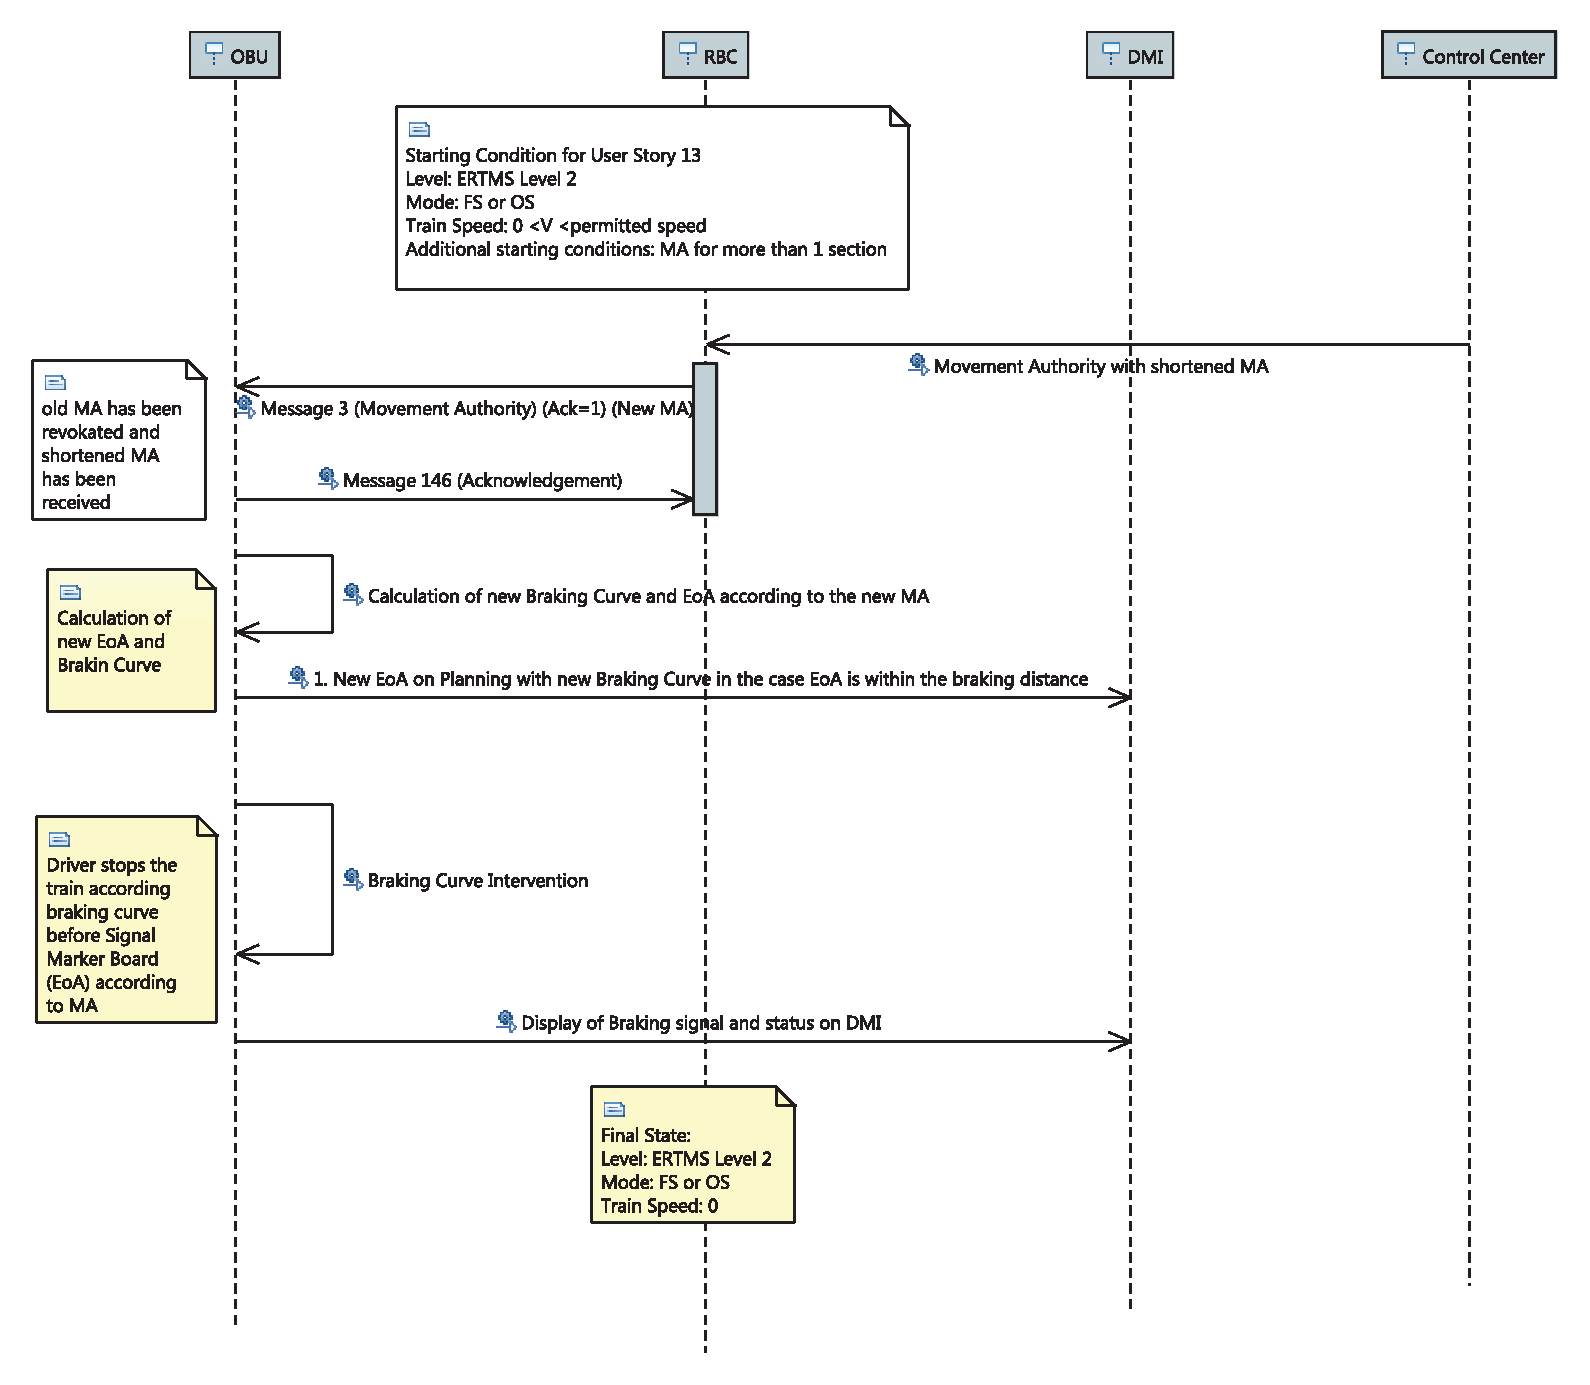
\includegraphics[width=6.5in]{images/UserStory13.eps}
  %\caption{Sequence Diagram for Use Case 13}
  %\label{fig:us13}
%\end{figure}

We had to solve the following task:

\begin{enumerate}
 \item Find a formal representation of the Amsterdam- Utrecht ETCS Level 2 line which allows validation of the Use Cases with the openETCS EVC- model in the loop
 \item Find an efficient way to model the test case scenarios
 \item Propose a concept which allows \emph{dynamic simulation}, meaning that we can actively drive a train, with a simulation environment that acts and reacts dynamically, instead of just providing playback of predefined scenarios.
\end {enumerate}



\section{The Amsterdam- Utrecht Reference Track}
\subsection{Introduction}

The openETCS Proof Of Concept is based on the Amsterdam- Utrecht ETCS line.\
It is one of the few ETCS lines that are already operational and where engineering and JRU data were available to the consortium.\newline
Some of the characteristics of the Amsterdam- Utrecht line  \cite{muttram08}.:
\begin{itemize}
 \item Four tracks
 \item Very busy mixed traffic
 \item ETCS Level 2 with mixed signalling, including wayside optical signals and ATB train protection for conventional traffic
 \item ERTMS 2.3.0 standard (Baseline 2)
\end{itemize}

For our Proof of Concept this means that, already in the "nominal scenarios", we see transitions from the conventional ATB train protection to ETCS L2 full supervision, that we need a representation of the balises found on the track, and a simple RBC model in order to act as a counterpart to the openETCS EVC model.

We had to decide to which level of fidelity we could model the track, and due to the focus of openETCS on the EVC reference design we limited the scope to building the simulation to "what the train can see".\newline
A full RBC model, the full set of operational rules as well as the interlocking logic are hence out of scope of this work.\newline


\subsection{Approach}

As an input, we had access to a set of engineering data, track layout plans, and selected JRU recordings from an ICE3 train of consortium member DB. Furthermore we could build on some initial modelling trials that were conducted by the consortium and on a comprehensive formalisation of the ETCS language, to be found at\newline https://github.com/openETCS/modeling/tree/master/model/Scade/System/ObuFunctions\newline .../ETCS\_Messaging/TrackMessages\newline
In addition we had access to a description of the operational rules for the Amsterdam- Utrecht line.
The first step to creating a dynamic simulation was the analysis of the available information, in order to have s old basis for our reverse- engineering effort.
\subsection{Engineering Data}
\subsubsection{Track Layout Plans}

\begin{figure}
  \centering
  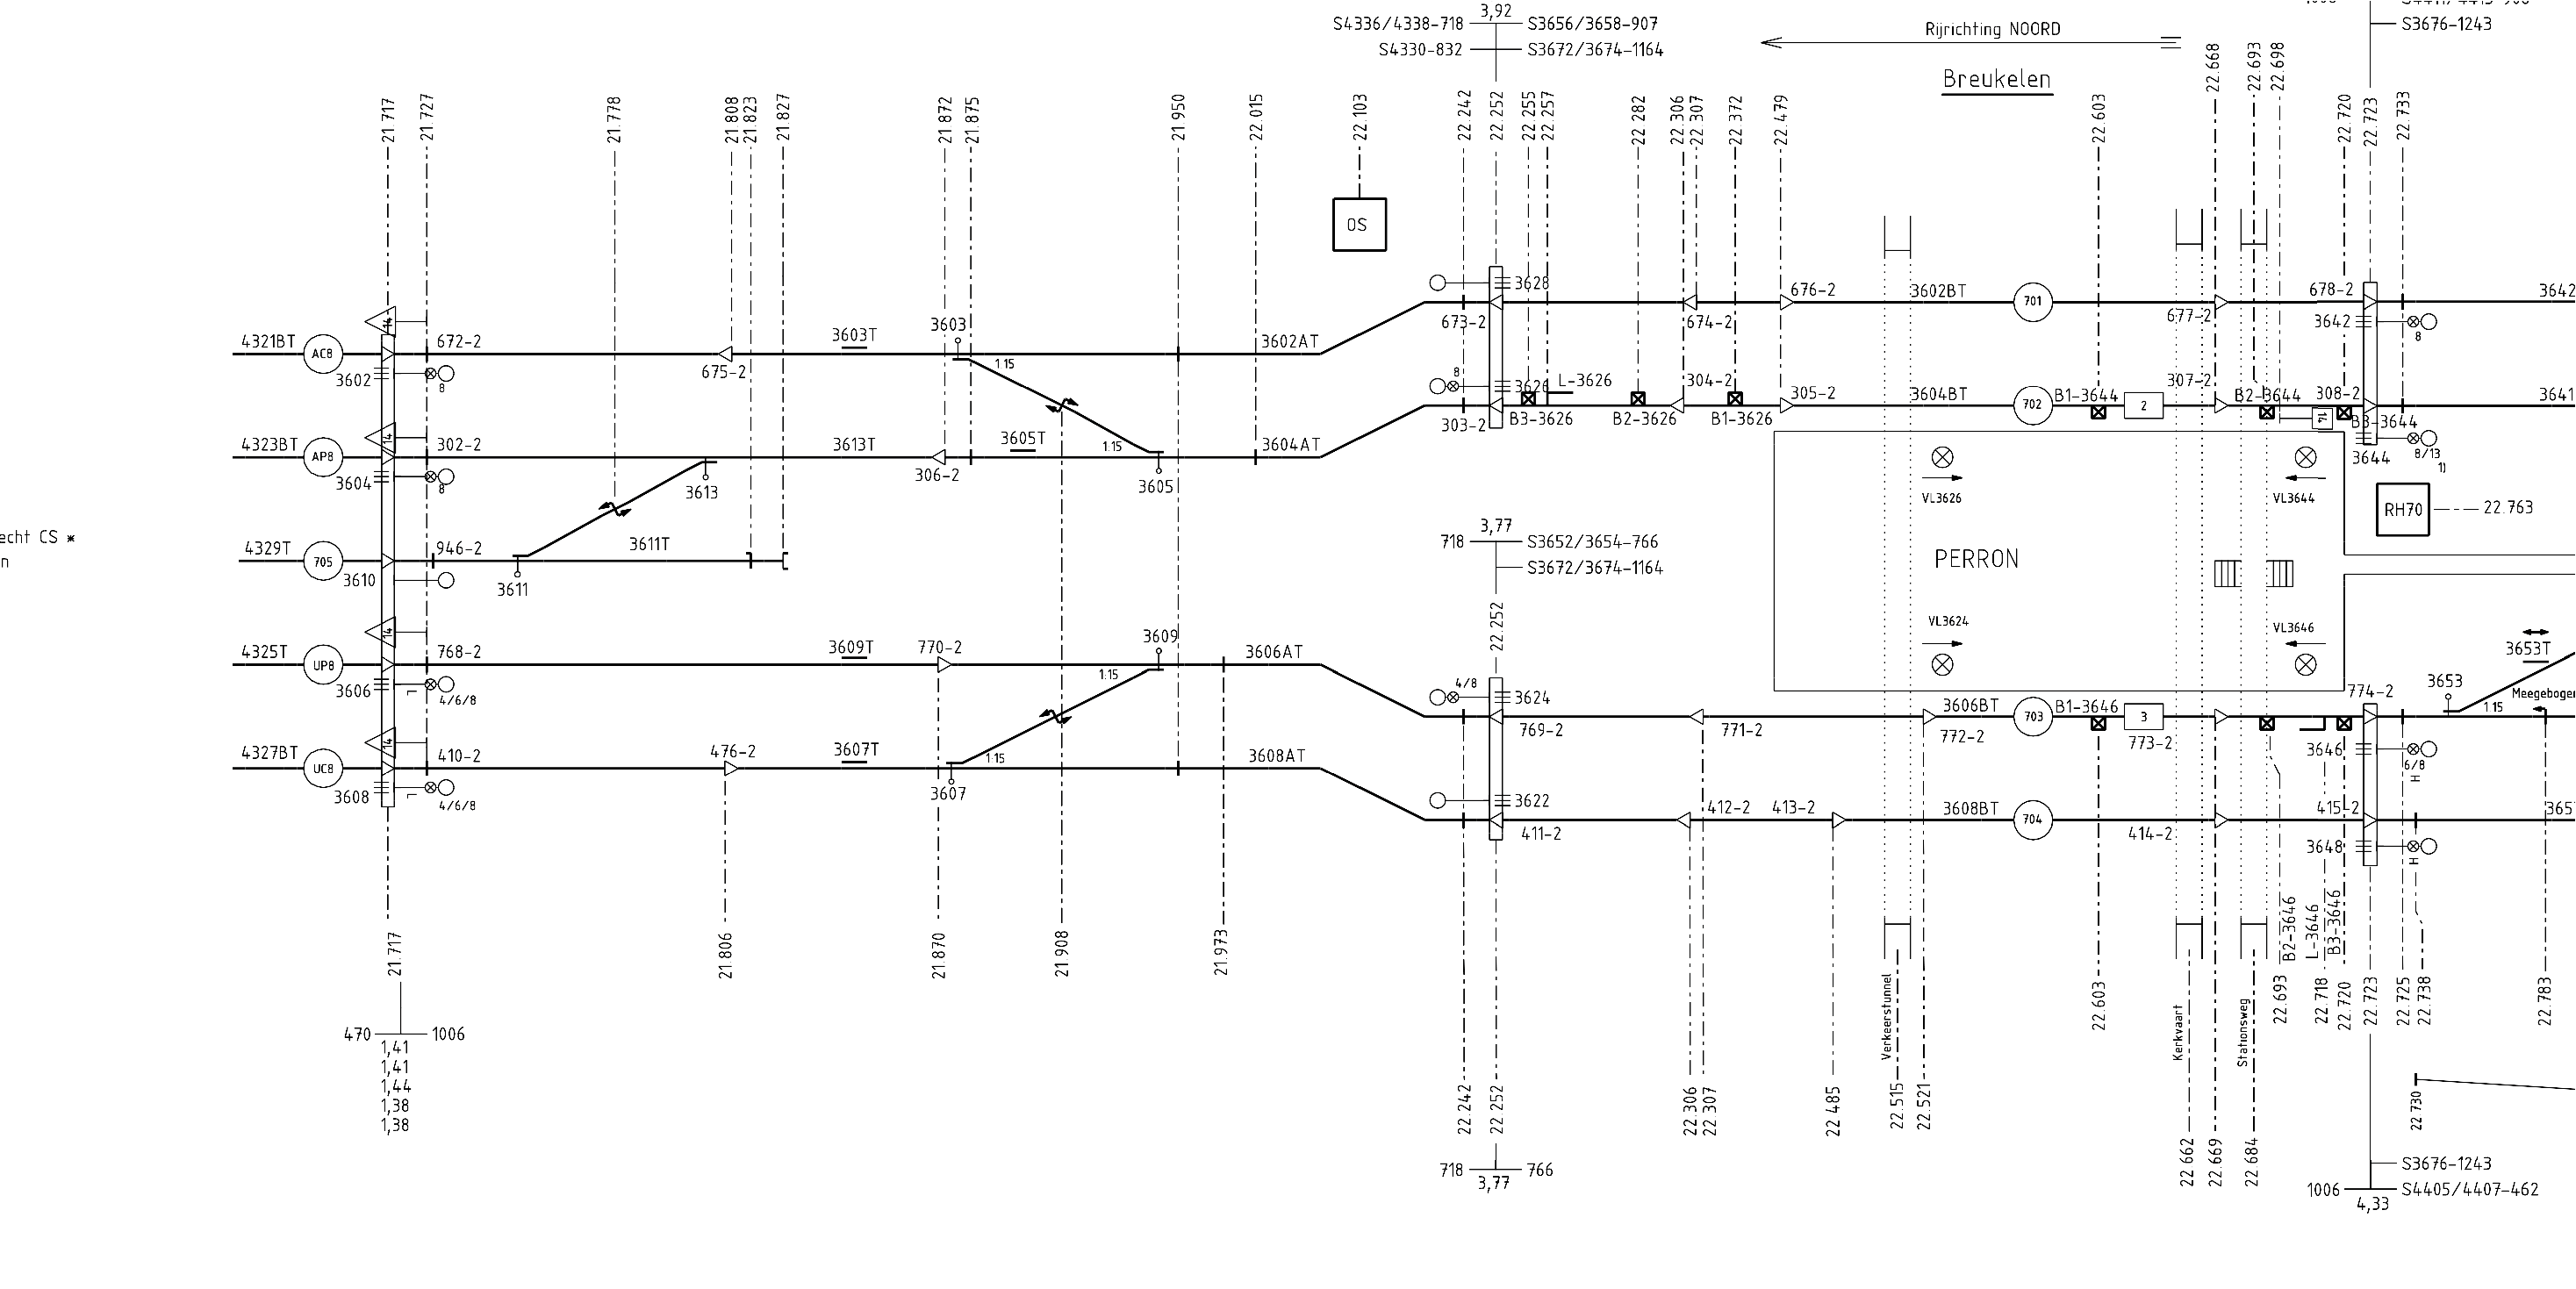
\includegraphics[angle=90, origin=c, width=4in]{images/Breukelen_Crop.eps}
  \caption{Example Track Layout Plan}
  \label{fig:breukelen}
\end{figure}

The definitive source of information for the balise positions were the track layout plans that do not only allow for a direct reading of the engineering positions of the balises, but also for an understanding of the actual situation on the track, the related signals, the points and stations etc. An example is given in figure \ref{fig:breukelen}.\newline



\subsubsection{Balise Position Data}

Table \ref {tab:balises} gives an example of engineering data as provided for positions and orientation of balises on the reference track.
The meaning of the columns is:
\begin{itemize}
 \item NID\_C: Country identifier of the track. The Amsterdam- Utrecht line has a NID\_C = 426 (Subset-026 7.5.1.86)\cite{SRS026-7}
 \item NID\_BG: Balise Group Identifier. (Subset-026 7.5.1.85)\cite{SRS026-7}
 \item Lint: Track section (not used for our model)
 \item km: Engineering location of the balise group. Please note that this position is the \emph{trackside view} of the balise group. The train is not aware of this absolute location reference.
 \item Or BG: Orientation of the balise group. The orientation is given with reference to the driving direction towards Amsterdam and Utrecht, respectively. A train driving in direction of Utrecht would see a balise group with orientation "Utrecht" as nominal, "Amsterdam" would be seen as "reverse".
 \item Or Line: Nominal direction of the track. "Z" means that the main direction of the track is southbound, which means towards Utrecht.
 \item Line No: Section number. Not used for our simulation.
 \end {itemize}

The full table is available in Appendix 1.

\begin{table}
  \centering
    \footnotesize\sffamily
\begin{tabular}{| l| l| l| r| l| l| l| l l}
\hline
\bf{NID\_C} & \bf{NID\_BG} & \bf{Lint} & \bf{km} & \bf{Or BG} & \bf{Or Line} & \bf{Line no} \\ 
\hline
426 & 352 & Asd-Asa & 105017 & Utrecht & Z & spoor UB \\
426 & 353 & Asd-Zvg & 1565 & Utrecht & Z & spoor UB \\
426 & 354 & Asd-Zvg & 3185 & Utrecht & Z & spoor UB \\
426 & 355 & Asd-Zvg & 4040 & Utrecht & Z & spoor UB \\
426 & 356 & Asd-Zvg & 4197 & Amsterdam & Z & spoor UB \\
426 & 357 & Asd-Zvg & 4252 & Amsterdam & Z & spoor 508 \\
426 & 358 & Asd-Zvg & 4428 & Amsterdam & Z & spoor 508 \\
426 & 359 & Asd-Zvg & 4598 & Utrecht & Z & spoor 508 \\
426 & 360 & Asd-Zvg & 4650 & Utrecht & Z & spoor 508 \\
426 & 361 & Asd-Zvg & 5083 & Amsterdam & Z & spoor 598 \\
426 & 362 & Asd-Zvg & 5137 & Amsterdam & Z & spoor 598 \\
426 & 363 & Asd-Zvg & 5372 & Utrecht & Z & spoor 598 \\
426 & 364 & Asd-Zvg & 5425 & Utrecht & Z & spoor 598 \\
426 & 365 & Asd-Zvg & 5598 & Amsterdam & Z & spoor 608 \\
426 & 366 & Asd-Zvg & 5649 & Amsterdam & Z & spoor 608 \\
426 & 367 & Asd-Zvg & 5805 & Amsterdam & Z & spoor 608 \\
426 & 368 & Asd-Zvg & 5945 & Utrecht & Z & spoor 608 \\
426 & 369 & Asd-Zvg & 6000 & Utrecht & Z & spoor 608 \\
426 & 370 & Asd-Zvg & 6940 & Amsterdam & Z & spoor UB1 \\
426 & 371 & Asd-Zvg & 6990 & Utrecht & Z & spoor UB1 \\
426 & 372 & Asd-Zvg & 7424 & Amsterdam & Z & spoor UB2 \\
426 & 373 & Asd-Zvg & 7625 & Amsterdam & Z & spoor UB2 \\
426 & 374 & Asd-Zvg & 7857 & Utrecht & Z & spoor UB2 \\
426 & 375 & Asd-Zvg & 8325 & Amsterdam & Z & spoor UB3 \\
426 & 376 & Asd-Zvg & 8774 & Amsterdam & Z & spoor UB3 \\
426 & 377 & Asd-Zvg & 9144 & Amsterdam & Z & spoor UB3 \\
\hline
\end{tabular}
\caption{Some balise positions in original format}
  \label{tab:balises}
\end{table}


\subsubsection{Message and Packet Data}

Message and Packet Data were not available as a set of engineering data. The project could however evaluate a set of JRU data from actual train passages on the Amsterdam- Utrecht corridor. One such data set was selected and used as a reference input for our balise and RBC message simulation.
The data were available in the form of annotated .csv files, which have been published on the Github repository as part of the User Story documentation.
As an example, we present in Table \ref{tab:p21} an instance of a packet 21 (Gradient Profile) which was sent as part of a Level2/3 Movement Authority Message. 

\begin{table}
  \footnotesize\sffamily
NID\_PACKET(8bits) = Gradient Profile(21)\newline
Q\_DIR(2bits) = Reverse(0)\newline
L\_PACKET(13bits) = 222bits(222)\newline
Q\_SCALE(2bits) = 1m(1)\newline
D\_GRADIENT(15bits) = 7890.0m(7890)\newline
Q\_GDIR(1bits) = Uphill(1)\newline
G\_A(8bits) = 2\textperthousand(2)\newline
N\_ITER(5bits) = 7(7)\newline
    1: D\_GRADIENT[1](15bits) = 220.0m(220)\newline
        Q\_GDIR[1](1bits) = Uphill(1)\newline
        G\_A[1](8bits) = 8\textperthousand(8)\newline
    2: D\_GRADIENT[2](15bits) = 420.0m(420)\newline
        Q\_GDIR[2](1bits) = Uphill(1)\newline
        G\_A[2](8bits) = 4\textperthousand(4)\newline
    3: D\_GRADIENT[3](15bits) = 140.0m(140)\newline
        Q\_GDIR[3](1bits) = Downhill(0)\newline
        G\_A[3](8bits) = 4\textperthousand(4)\newline
    4: D\_GRADIENT[4](15bits) = 120.0m(120)\newline
        Q\_GDIR[4](1bits) = Downhill(0)\newline
        G\_A[4](8bits) = 12\textperthousand(12)\newline
    5: D\_GRADIENT[5](15bits) = 320.0m(320)\newline
        Q\_GDIR[5](1bits) = Downhill(0)\newline
        G\_A[5](8bits) = 5\textperthousand(5)\newline
    6: D\_GRADIENT[6](15bits) = 110.0m(110)\newline
        Q\_GDIR[6](1bits) = Uphill(1)\newline
        G\_A[6](8bits) = 2\textperthousand(2)\newline
    7: D\_GRADIENT[7](15bits) = 178.0m(178)\newline
        Q\_GDIR[7](1bits) = Uphill(1)\newline
        G\_A[7](8bits) = End of gradient profile(255)"\newline
\caption{Example packet data for Gradient Profile as found in the JRU log}
  \label{tab:p21}
\end{table}

A full description of the packet definition can be found in Subset-026 (7.4.2.6) \cite {SRS026-7}. The actual semantics of the packet are not interesting for us. Our only task is to interpret them in the right way so that they will be correctly decoded once they reach the EVC model.\newline
In order to avoid transcription errors, we want to use the data from the JRU trace "as raw as possible".  For that purpose, a detailed analysis of the contents of this log file is required:
The file is a result of a script interpreting the raw data: bits are converted to integers, and some comments are added.
If we take the first line of the packet:
\begin{table}[H]
  \footnotesize\sffamily
NID\_PACKET(8bits) = Gradient Profile(21)
\end{table}
Here, we can easily understand that in the original packet (bitstream), the value used 8 bits, and has been interpreted as decimal number (21).
If we take another line, the interpretation is equally straightforward:
\begin{table}[H]
  \footnotesize\sffamily
D\_GRADIENT(15bits) = 7890.0m(7890)
\end{table}
We could easily say that there is a 1:1 translation of the real value (7890.0m) and the representation found in the JRU data (7890).
However, this is only due to the following line:
\begin{table}[H]
  \footnotesize\sffamily
Q\_SCALE(2bits) = 1m(1)
\end{table}
which just means that the values for distance have to be scale with a factor of 1m.

If we look at packet 27 (international static speed profile), we can see another interesting aspect:

\begin{table}[H]
  \footnotesize\sffamily
NID\_PACKET(8bits) = International Static Speed Profile(27) \\
Q\_DIR(2bits) = Reverse(0) \\
L\_PACKET(13bits) = 86bits(86) \\
Q\_SCALE(2bits) = 1m(1) \\
D\_STATIC(15bits) = 7890.0m(7890) \\
V\_STATIC(7bits) = 160km/h(32) \\
Q\_FRONT(1bits) = Train length delay on validity end point(0) \\
N\_ITER(5bits) = 0(0) \\
N\_ITER(5bits) = 1(1) \\
    1: D\_STATIC[1](15bits) = 1508.0m(1508) \\
        V\_STATIC[1](7bits) = End of SSP(127) \\
        Q\_FRONT[1](1bits) = Train length delay on validity end point(0) \\
        N\_ITER[1](5bits) = 0(0)" \\
\caption{Example packet data for Speed Profile as found in the JRU log}
  \label{tab:p27}
\end{table}

Looking at the line:
\begin{table}[H]
  \footnotesize\sffamily
V\_STATIC(7bits) = 160km/h(32) \\
\end{table}
we can see that the representation in the JRU log (32) and its interpretation (160km/h) do not have the same scale. 
\cite{SRS026-7} (7.5.1.171) gives the following information:
\begin{figure}[H]
  \centering
  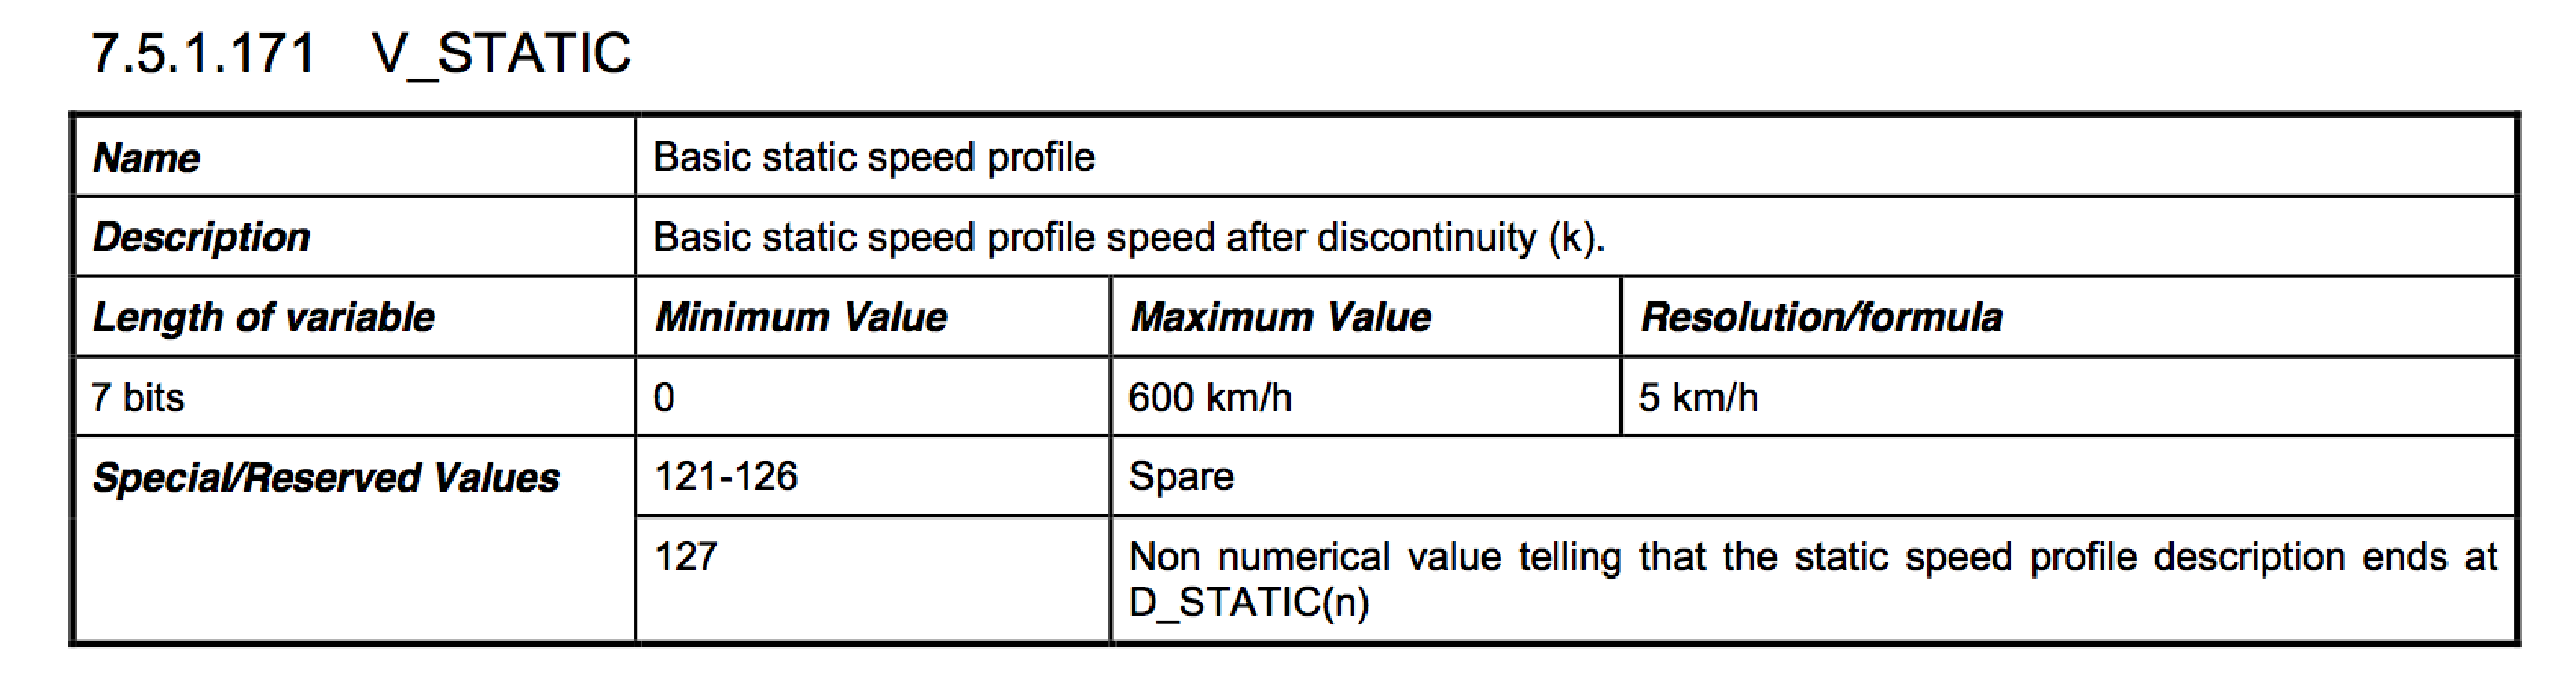
\includegraphics[ width=6in]{images/V-STATIC.eps}
  \caption{Variable definition for V\_STATIC}
  \label{fig:vstatic}
\end{figure}
This means that V\_STATIC is using a scaling factor of 5 to encode the speed.\newline

We conclude, that in general, we will provide a track simulation model (balises positions, messages and packets) containing the \emph{integer representation} as found in the JRU log. We will rely on the TrackMessages library to correctly translate the values into the proper scaling for use onboard the EVC.
Initially this decision was only taken in order to reduce room for interpretation/ transcription errors when building the track simulation model, however, in context of WP5 (Demonstrator) this decision has proven to be very valuable, as it created a requirement for development of a full formalisation of Subset-026, Chapters 6, 7, and 8.


\subsection{Operational Rules}

As a reference, we had access to the operational rules for the Amsterdam- Utrecht corridor \cite{OpRules}. Due to the limited scope of the project, we did not attempt to create simulation models based on this document, we rather used it a means to validate our model.\newline
Future work, possibly in the following months of this project, may include some basic research on formalisation of such operational rules.\newline


\section{Simulation Concepts}
\subsection{The State of The Art in Railway (ETCS) simulation}

The ETCS requirements provides extensive specification on test formats and a test environment, for example in Subset-076 and Subset-094.
Current ETCS Simulation Environments allow to:
\begin{itemize}
 \item Use a set of offline tools to prepare track and scenario data 
 \item Run a train through the hardcoded scenarios, interacting with the (real or simulated) EVC and accepting input from a driver
 \item Use a simulated EVC
 \item Use a simulated DMI (Driver Machine Interface)
 \item Emit messages, packets and telegrams (priorly prepared) through a trackside simulator
\end{itemize}
 
openETCS is aiming in providing an \emph{open, formal executable specification of the EVC kernel}, in order to serve as a functional reference and as a basis for working on novel approaches for interoperability.

We therefore require a simulation concept that supports the development, validation and maintenance of this openETCS kernel, and complements it also after the completion of this project. Some objectives we identified were:
\begin{itemize}
 \item \emph{Dynamic Behaviour}: The trackside simulation should be able to actively act and react. In other words, instead of reacting to predefined scenarios, all input parameters should be independent of each other. 
 \item The approach should allow \emph{blackbox} as well as \emph{whitebox} simulation.
 \item The simulation model should allow certification as a verification tool (in the context of EN50128)
 \item The system should be hardware- independent
 \item The system should at least cover all functionality of the current state of the art
 \item The approach should allow deployment through all phases of EVC and track development, testing and validation, including the development of the openETCS kernel itself.
\end{itemize}
 
\subsection{Dynamic track simulation throughout the (open)ETCS lifecycle}
Our concept is aiming at covering all aspects of verification and validation throughout the openETCS lifecycle, and in the lifecycle of ETCS onboard and trackside installations in general.\newline Not all points are relevant for openETCS, but rather lay the grounds for ongoing work of the openETCS foundation and for industrial exploitation.

\subsubsection{User Validation}

The term \emph{User Validation} refers to the practice to use simplified simulation models during the day-to-day analysis and development work.\newline
openETCS is using SCADE Suite as standard development tool.\newline During system analysis and development cycle, each SCADE user can iteratively cycle through analysis / design/ simulation in order to understand the requirements, model them, and functionally validate them. This approach strongly supports the distributed and agile openETCS process. \newline Where appropriate, users can integrate the track simulation model, fully, or in part, in their development cycle.

\subsubsection{openETCS system integration}

openETCS system integration can be grouped into two main issues:
\begin{enumerate}
 \item Integration of the various parts of the openETCS EVC kernel (Figure \ref{fig:Alstom1} provides an example of an EVC functional breakdown)
\begin{figure}[H]
  \centering
  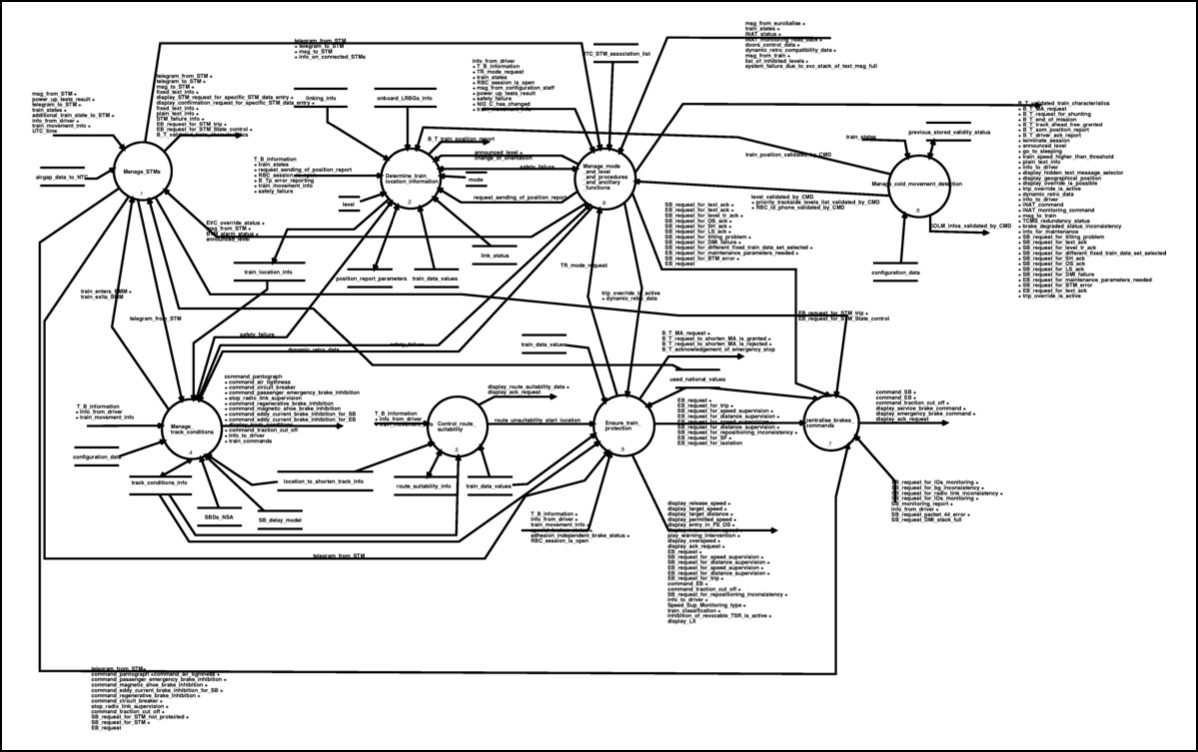
\includegraphics[width=6in]{images/AlstomDF.eps}
  \caption{Overview of Components in the ALSTOM EVC architecture, using TeamWork SA RT notation}
  \label{fig:Alstom1}
\end{figure}
 \item Integration of the different modules of the Proof of Concept. (Figure \ref{fig:POC} shows the user interface of the environment used to integrate the different elements of the Proof of Concept)
During the 3rd iteration effort of openETCS, a model- level integration environment was created. It includes, on model level, the following elements:
\begin{enumerate}
 \item The openETCS EVC kernel formal model
 \item The openETCS DMI formal model
 \item A simple environment toolbox, containing a train model, odometry model, and a telegram/ packet generator
 \item A boilerplate to interact with the system (driver inputs, graphical outputs)
\end{enumerate}
 \begin{figure}[H]
  \centering
  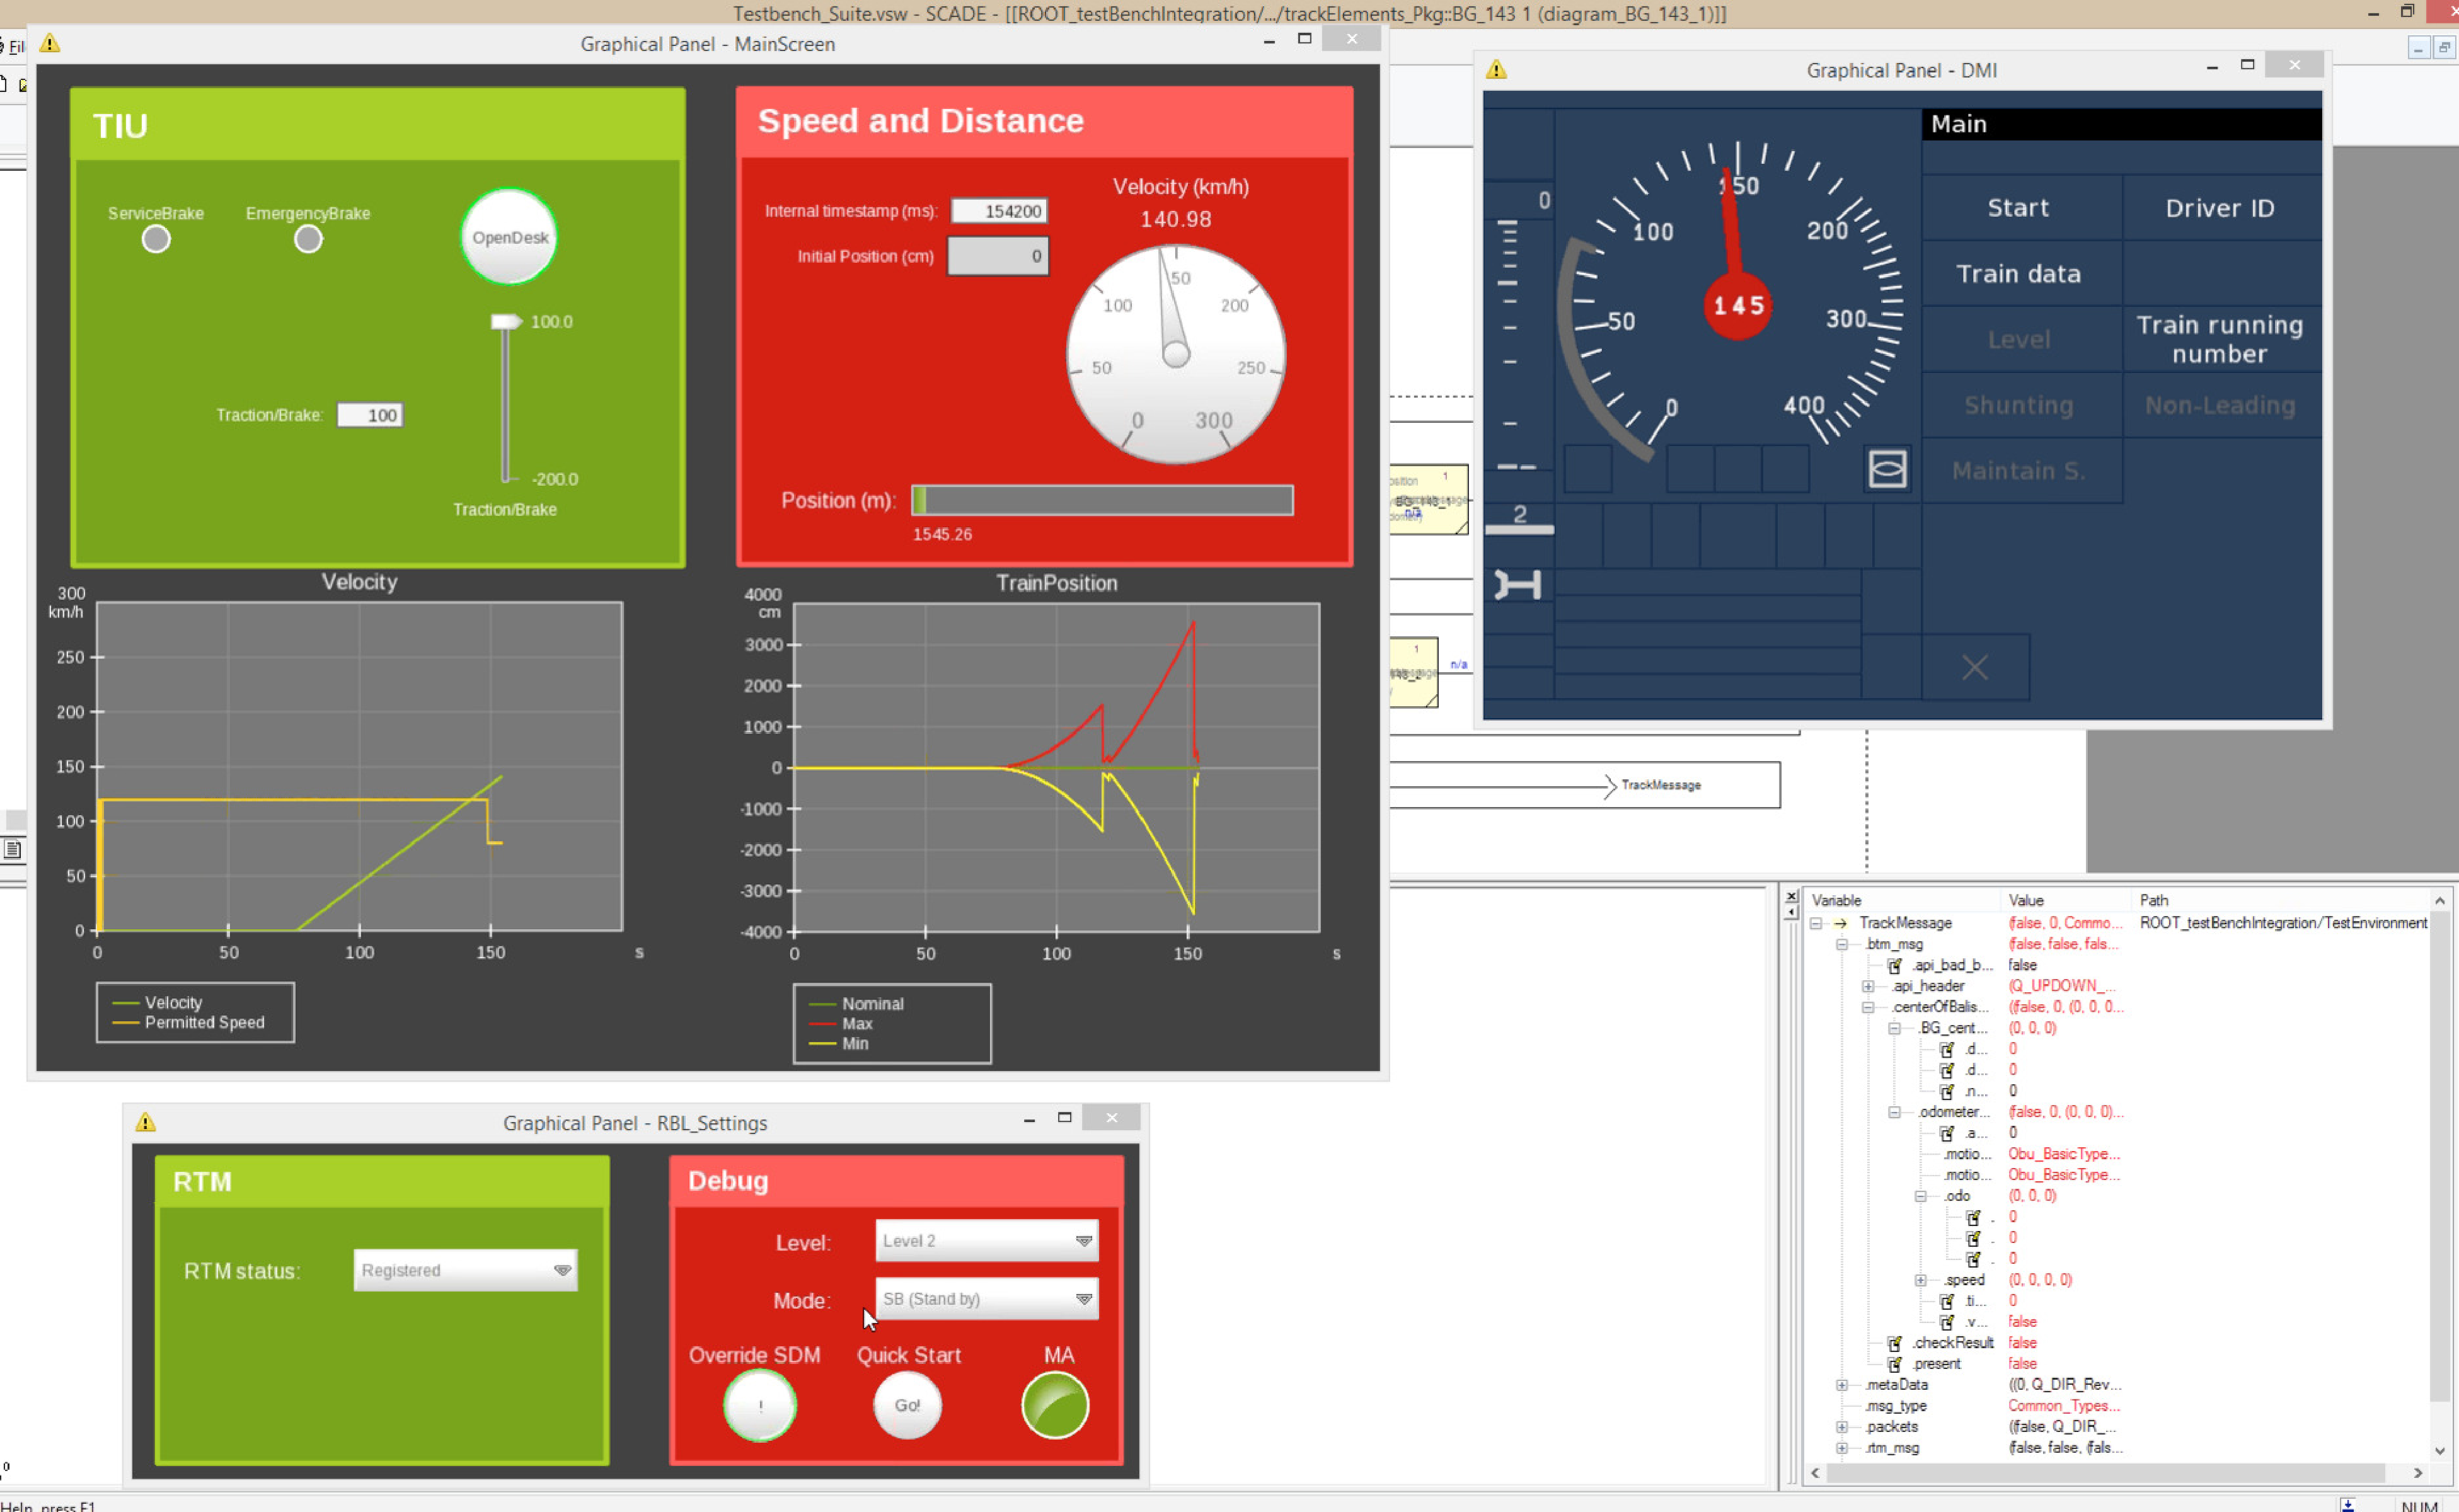
\includegraphics[width=6in]{images/POC_environment.eps}
  \caption{Depiction of the openETCS Third Iteration Proof of Concept Environment}
  \label{fig:POC}
\end{figure}
For the full Proof of Concept, the complete track model is being integrated into the integration environment, allowing to develop, validate and demonstrate the Use Cases.
\end{enumerate}



\subsection{The role of dynamic simulation in the formalisation of ERA ETCS Change Requests and in improving interoperability}

The complexity of the ETCS software requirements specification and it's history of incremental changes make for its reputation to lacking stringency, consistency and a clear, unified concept. 
The original objective of a unique set of requirements that, if only correctly implemented, would guarantee interoperability, looks quite utopian.
At best, there is a common syntax, but there is no common grammar, as far as the interactions between trackside and onboard are concerned.\newline
openETCS's original concept has addressed the main problem of ETCS by building an openly available formal model, which is a possible basis for a formalisation of the ERA ETCS change request process.
\begin{figure}
 \centering
  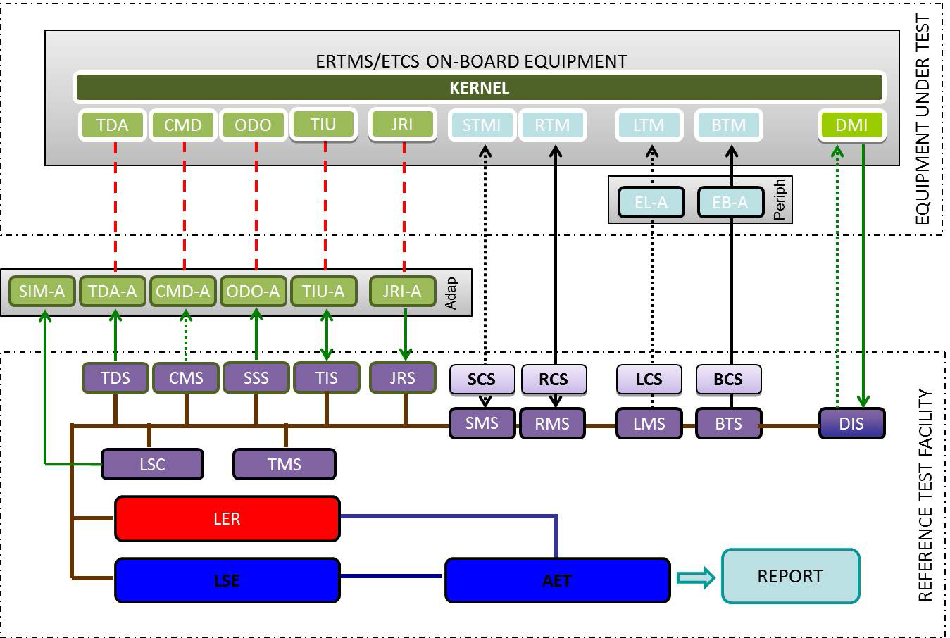
\includegraphics[width=6in]{images/SUBSET-094-v300-3-overview.eps}
  \caption{Reference test architecture for ERTMS/ETCS on-board equipment}
   \label{fig:Subs94}
\end{figure}


Subset-94 \cite{Subset094}, see Fig. \ref{fig:Subs94} describes functional requirements for an on-board Reference Test Facility. In section 5.1.1.1 it states \emph{"The test architecture described in this document is focused on performing the tests defined in Subset-076-6-3 (...), and hence, the compliance with Subset-026"} In consequence this would mean that if any ETCS Onboard Unit would pass the tests as described in Subset-076 \cite{Subset076} on an on-board Reference Test Facility, it should work on any validated ETCS infrastructure, which is not really the case.

We believe that providing a formal model of the onboard functionality is only half of the solution: It needs to be complemented by a formal model of the trackside functionality. The validation of the onboard against Subset-076 and the other relevant standards referenced in the CCS TSI is not sufficient, we need to harmonise the onboard and the track \emph{before} we start the actual (real- world) track implementation. Only that way we can reduce the effort and make progress towards the goal of "Zero Onsite Testing".

\begin{figure}[H]
 \centering
  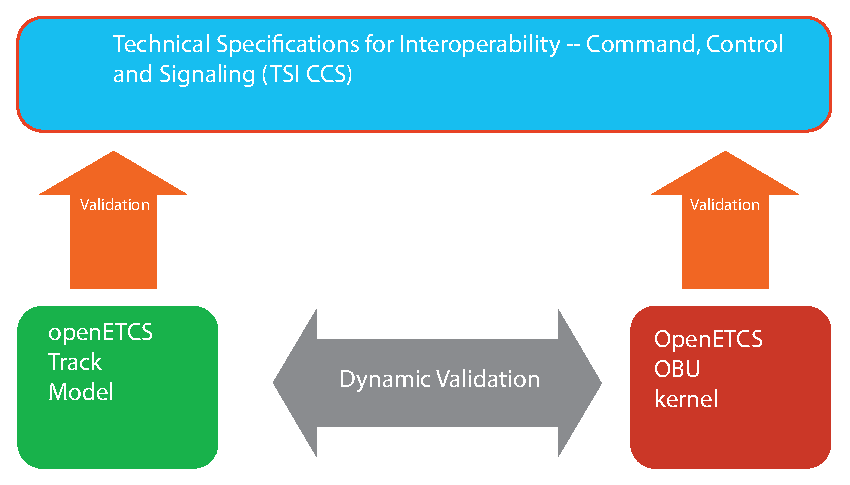
\includegraphics[width=4in]{images/DynamicSimulationForInterOp.eps}
  \caption{Dynamic simulation for improving interoperability}
   \label{fig:InterOpDynSim}
\end{figure}

The validation against the relevant standards referenced in the Document "Applicable standards in HS Control-Command and Signalling TSI (2006/860/EC)" \cite{CCS-TSI} is complemented by extensive validation using the co-simulation of the openETCS formal, executable specifications for the trackside and the onboard functionalities. 

As a first step, a validation process for the formal track model must be established. 


\subsubsection{Validation of the openETCS Dynamic Simulation Model against the existing, scenario- based test cases for the Reference Track}

During the analysis and design phase of openETCS, the Track Model is being validated by WP4. We have taken care that the basic interface concepts and data structures at the component boundaries are compatible with the standard approaches as described in Subset-076 \cite{Subset076} and Subset-094 \cite{Subset094}, however such integration is beyond the scope of this work.\newline 
WP4 is validating the Track Model against the script- driven simulation scenarios used by the team members of work package 4. In addition, peer review is being provided by WP4.\newline
The objective of this exercise is to ensure equal behaviour of the dynamic simulation model as compared to the conventional approach, as far as appropriate. 

\subsubsection{Checking the track model's consistency by comparing engineering data and packet data}

During analysis of the initial Track Model, some discrepancies between the balise positions as defined in the engineering data and the related data concerning linking distance as recorded in the JRU have been discovered. We created a cross reference file (see Table \ref{tab:xrefbalises}) using a spreadsheet tool. 

The columns must be read as follows:
\begin{itemize}
 \item NID\_C: Country identifier of the track. The Amsterdam- Utrecht line has a NID\_C = 426 (Subset-026 7.5.1.86)\cite{SRS026-7}
 \item NID\_BG: Balise Group Identifier. (Subset-026 7.5.1.85)\cite{SRS026-7}
 \item Corrected pos.: Engineering position \emph{after correction} based on linking data (in Meters)
 \item Difference: Difference (in Meters) between the engineering position and the corrected position (positive numbers move the balise group down the track, e.g. towards Utrecht)
 \item Or: Orientation of the Balise Group as defined in the engineering data
 \item Or US: Orientation of the Balise Group from the train's perspective as it runs from Amsterdam towards Utrecht, as defined in the User Stories (=US)
 \item Packets: Packets emitted from a particular Balise Group 
\end{itemize}


\begin{longtable}{|r |r |r |r |l |l |l |}
\hline
NID\_C & NID\_BG & Corrected pos.  & Difference  & Or & Or US & Packets \\
\hline
\endfirsthead
\hline
NID\_C & NID\_BG & Corrected pos.  & Difference  & Or & Or US & Packets \\
\hline
\endhead
\hline
\multicolumn{7}{r}{{Continued next page\ldots}} \
\endfoot
\hline
\caption{Cross reference table for the balise groups relevant for the Proof of Concept}
  \label{tab:xrefbalises}
\endlastfoot


426 & 352 &  &  & Utrecht & nominal & P45 \\
426 & 353 &  &  & Utrecht & nominal & P42 \\
426 & 354 & 3185 & 0 & Utrecht & nominal & P42,P46,P46,P3 \\
426 & 351 & 3997 & 2 & Utrecht & nominal & none \\
426 & 355 & 4051 & 11 & Utrecht & nominal & P42,P46 \\
426 & 356 & 4205 & 8 & Amsterdam & reverse & P41 \\
426 & 357 & 4255 & 3 & Amsterdam & reverse & none \\
426 & 358 & 4430 & 2 & Amsterdam & reverse & none \\
426 & 359 & 4599 & 1 & Utrecht & nominal & none \\
426 & 360 & 4654 & 4 & Utrecht & nominal & P137 \\
426 & 361 & 5082 & -1 & Amsterdam & reverse & none \\
426 & 362 & 5136 & -1 & Amsterdam & reverse & none \\
426 & 363 & 5374 & 2 & Utrecht & nominal & none \\
426 & 364 & 5428 & 3 & Utrecht & nominal & none \\
426 & 365 & 5600 & 2 & Amsterdam & reverse & none \\
426 & 366 & 5655 & 6 & Amsterdam & reverse & none \\
426 & 367 & 5807 & 2 & Amsterdam & reverse & none \\
426 & 368 & 5948 & 3 & Utrecht & nominal & none \\
426 & 369 & 6001 & 1 & Utrecht & nominal & P137 \\
426 & 341 & 6472 & 2 & Amsterdam & reverse & none \\
426 & 370 & 6940 & 0 & Amsterdam & reverse & none \\
426 & 371 & 6993 & 3 & Utrecht & nominal & none \\
426 & 372 & 7426 & 2 & Amsterdam & reverse & none \\
426 & 373 & 7626 & 1 & Amsterdam & reverse & none \\
426 & 374 & 7858 & 1 & Utrecht & nominal & none \\
426 & 375 & 8326 & 1 & Amsterdam & reverse & none \\
426 & 376 & 8775 & 1 & Amsterdam & reverse & none \\
426 & 377 & 9146 & 2 & Amsterdam & reverse & none \\
426 & 378 & 9561 & 3 & Utrecht & nominal & none \\
426 & 379 & 9615 & 3 & Utrecht & nominal & none \\
426 & 380 & 9842 & 1 & Amsterdam & reverse & none \\
426 & 381 & 9896 & 3 & Amsterdam & reverse & none \\
426 & 382 & 10096 & 3 & Amsterdam & reverse & none \\
426 & 383 & 10596 & 4 & Amsterdam & reverse & none \\
426 & 384 & 11026 & 4 & Utrecht & nominal & none \\
426 & 385 & 11091 & 7 & Utrecht & nominal & none \\
426 & 386 & 11280 & 5 & Amsterdam & reverse & none \\
426 & 387 & 11334 & 5 & Amsterdam & reverse & none \\
426 & 388 & 11834 & 7 & Amsterdam & reverse & none \\
426 & 389 & 12582 & 12 & Utrecht & nominal & none \\
426 & 390 & 12689 & 11 & Amsterdam & reverse & none \\
426 & 391 & 13190 & 12 & Amsterdam & reverse & none \\
426 & 392 & 14064 & 7 & Utrecht & nominal & none \\
426 & 393 & 14172 & 6 & Amsterdam & reverse & none \\
426 & 394 & 14879 & 2 & Amsterdam & reverse & none \\
426 & 395 & 15575 & -2 & Utrecht & nominal & none \\
426 & 396 & 15684 & -2 & Amsterdam & reverse & none \\
426 & 397 & 16376 & -3 & Utrecht & nominal & none \\
426 & 398 & 17075 & -4 & Utrecht & nominal & none \\
426 & 399 & 17202 & -9 & Amsterdam & reverse & none \\
426 & 400 & 17820 & -4 & Utrecht & nominal & none \\
426 & 401 & 18432 & -4 & Utrecht & nominal & none \\
426 & 402 & 18737 & -1 & Amsterdam & reverse & none \\
426 & 403 & 19327 & 0 & Utrecht & nominal & none \\
426 & 404 & 19891 & 2 & Utrecht & nominal & none \\
426 & 405 & 20230 & 3 & Amsterdam & reverse & none \\
426 & 406 & 20749 & 4 & Utrecht & nominal & none \\
426 & 407 & 21198 & 6 & Utrecht & nominal & none \\
426 & 408 & 21594 & 6 & Amsterdam & reverse & none \\
426 & 409 & 21669 & 6 & Utrecht & nominal & none \\
426 & 410 & 21723 & 6 & Utrecht & nominal & none \\
426 & 476 & 21813 & 7 & Utrecht & nominal & none \\
426 & 411 & 22258 & 6 & Amsterdam & reverse & none \\
426 & 412 & 22313 & 7 & Amsterdam & reverse & none \\
426 & 413 & 22494 & 9 & Utrecht & nominal & none \\
426 & 414 & 22681 & 12 & Utrecht & nominal & none \\
426 & 415 & 22734 & 11 & Utrecht & nominal & none \\
426 & 416 & 23032 & 13 & Amsterdam & reverse & none \\
426 & 417 & 23086 & 15 & Amsterdam & reverse & none \\
426 & 418 & 23146 & 14 & Utrecht & nominal & none \\
426 & 419 & 23957 & 22 & Amsterdam & reverse & none \\
426 & 420 & 24505 & 30 & Utrecht & nominal & none \\
426 & 421 & 25291 & 36 & Amsterdam & reverse & none \\
426 & 422 & 25934 & 34 & Utrecht & nominal & none \\
426 & 423 & 26453 & 33 & Amsterdam & reverse & none \\
426 & 424 & 27245 & 35 & Utrecht & nominal & none \\
426 & 425 & 27311 & 33 & Utrecht & nominal & none \\
426 & 426 & 27558 & 33 & Amsterdam & reverse & none \\
426 & 427 & 27612 & 34 & Amsterdam & reverse & none \\
426 & 428 & 27783 & 35 & Utrecht & nominal & none \\
426 & 429 & 28121 & 35 & Amsterdam & reverse & none \\
426 & 477 & 28460 & 36 & Utrecht & nominal & none \\
426 & 430 & 28760 & 33 & Utrecht & nominal & none \\
426 & 431 & 28814 & 35 & Utrecht & nominal & none \\
426 & 432 & 29289 & 34 & Amsterdam & reverse & none \\
426 & 433 & 29343 & 32 & Amsterdam & reverse & none \\
426 & 434 & 29412 & 34 & Utrecht & nominal & none \\
426 & 435 & 29466 & 32 & Utrecht & nominal & none \\
426 & 436 & 29691 & 30 & Amsterdam & reverse & none \\
426 & 437 & 29757 & 31 & Amsterdam & reverse & none \\
426 & 438 & 30565 & 31 & Utrecht & nominal & none \\
426 & 439 & 30794 & 31 & Amsterdam & reverse & none \\
426 & 440 & 31502 & 32 & Utrecht & nominal & none \\
426 & 441 & 32165 & 31 & Amsterdam & reverse & none \\
426 & 442 & 32327 & 32 & Utrecht & nominal & none \\
426 & 443 & 32381 & 31 & Utrecht & nominal & none \\
426 & 444 & 32867 & 32 & Amsterdam & reverse & none \\
426 & 445 & 32921 & 34 & Amsterdam & reverse & none \\
\end{longtable}

We assumed the JRU data to be more accurate than the original engineering data, as the Amsterdam- Utrecht track is already operational and the packet data must therefore be considered as definitive.

Note: \emph{As the Balise Groups with NID\_BG 352 and 353 are not linked, no correction data are applicable.}

\subsubsection{Validation of the openETCS EVC kernel against the reference track}

Once the reference track model is considered to correctly reflect the infrastructure and events as recorded for the "real" reference track, it can be used to validate the functionality of the openETCS kernel against the reference track, as depicted in Figure \ref{fig:InterOpDynSim} above.\newline Once this achieved, we can consider the Reference Track Model and the Reference ETCS kernel to be interoperable, at least to the extent that the User Stories cover the actual operational situation on the track.\newline Extending this approach to full CCS TSI coverage would assure that both the Track and the EVC models are TSI compliant, and they are interoperable as well.\newline \newline
\emph{Within the openETCS effort, we will limit our efforts to demonstrating functional interoperability between the reference track and onboard.}


\subsubsection{Validation of tracks and OBUs against the openETCS reference EVC}

openETCS has claimed as on if its main objectives to create a \emph{Reference ETCS Kernel}, against which future onboard system may be validated.\newline We intend to extend this concept to validating new Dynamic Track Models against the openETCS kernel as well, with the ultimate objective to have a library of validated tracks against which future Onboard Unit implementations can be tested.\newline \newline
\emph{The extension of the validation concept beyond the current reference track model for the Amsterdam- Utrecht corridor is beyond the scope of the openETCS effort.}
 
\subsubsection{Verification and Validation in an EN50128 SIL4 context}

openETCS has chosen the SCADE\footnote{SCADE = Safety Critical Application Development Environment}  Suite from Esterel Technologies as software development tool. The rationale behind this decision was to enable a future development of a CENELEC EN 50128 SIL4\footnote{European Committee for Electrotechnical Standardization standard for Safety Critical Software Development in Railways, Safety Integrity Level 4} compliant ETCS reference kernel.\newline We decided to use the same development environment for the Track Model. This will enable us to certify the Track Model (and the process to create such models) in EN50128 context, meaning that it can be used as basis for a trusted and certified verification and validation tool suite.\newline \newline
\emph{Process definition and certification are beyond the scope of openETCS. We will concentrate on demonstrating functional aspects.}

\subsubsection{Transferring the concept to WP5 (Demonstrator)}

As we can generate C- code from the Track Model, it is also possible to embed the Track Model into external simulation and testing environments.  As a first trial, we have generated code for the model and embedded it onto a Raspberry Pi2 hardware, which can be coupled to WP5 demonstrator hardware via Ethernet. (See figure \ref{fig:raspb})\newline Of course, the generated code can also easily be integrated on any other hardware platform. Thanks to the cycle- based execution model of SCADE, this is very straightforward.

\begin{figure}[H]
  \centering
  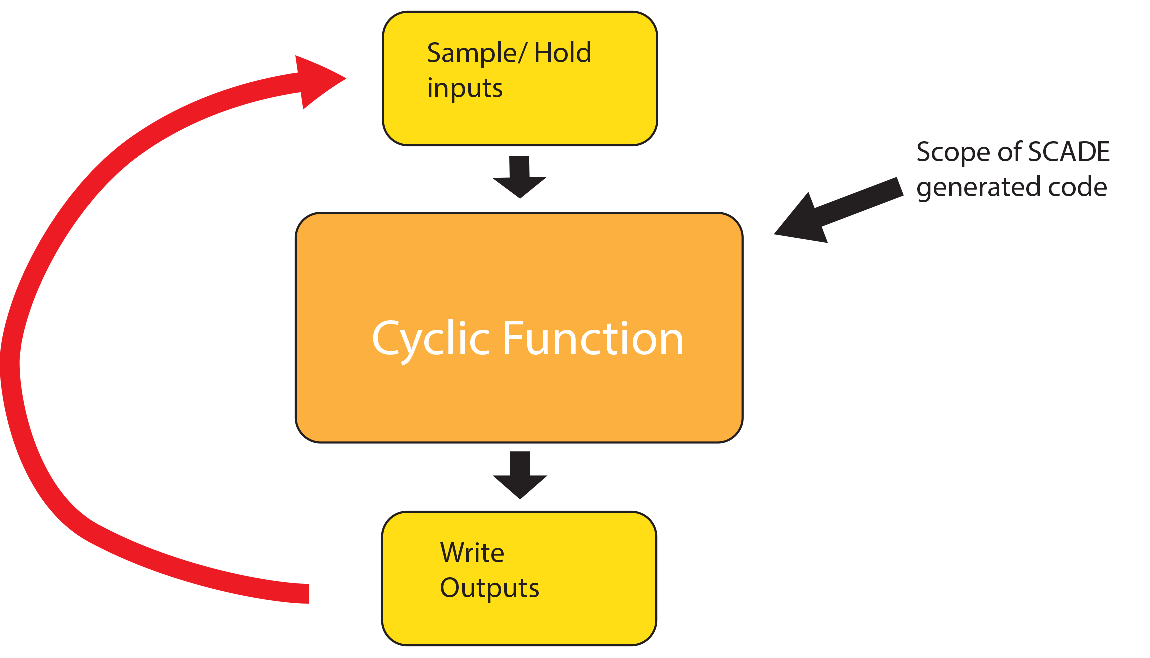
\includegraphics[width=4in]{images/cyclscade.eps}
  \caption{SCADE cycle- based execution model}
  \label{fig:SCcycle}
\end{figure}

The cyclic function contains the complete Track Model. 
\begin{figure}
  \centering
  \includegraphics[width=4in]{images/Raspberry.pdf}
  \caption{Raspberry Pi2 running the track model}
   % picture by LEA Railergy^	, licensed under CC BY-SA 3.0
  \label{fig:raspb}
\end{figure}

\newpage

\section{Formal model for trackside simulation}
\subsection{Simulation concept}

The simulation of the track can be seen as an integral part of a simulation and validation facility. While, at the moment, the openETCS demonstration environment is not designed to be Subset-094 compliant, it's basic concept is similar and extension to a full onboard- unit test facility is possible in the future.\newline
\begin{figure}[H]
  \centering
  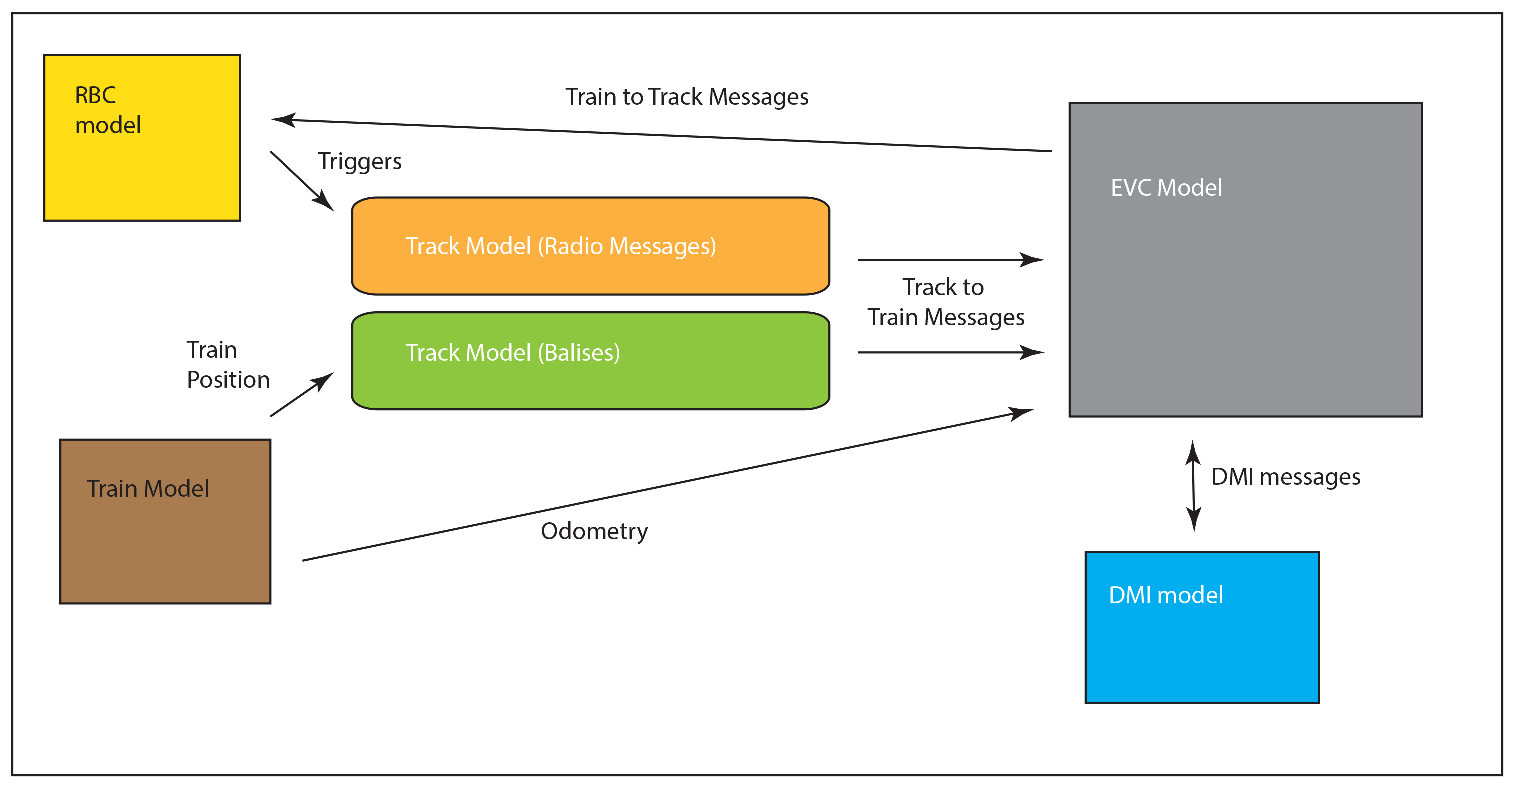
\includegraphics[width=6in]{images/SimArch.eps}
  \caption{Simplified Simulation Concept}
  \label{fig:simconcept}
\end{figure}


\subsubsection{Scope of the model}

The scope of the model is defined by the User Stories. A full balise and RBC model exists for the southbound track of the western pair of tracks on the Amsterdam- Utrecht corridor, between the stations Amsterdam Amstel and Utrecht CS.

\subsubsection{Overview}

The Track Model consists of two main parts:
\begin{itemize}
 \item The balise model:
  \begin{itemize} 
   \item The balise model receives a single input from the \emph{train model}, which provides information on the nominal train position.
   \item The balise model sends messages and packets to the \emph{EVC Model} when the train passes a position where a balise is located
  \end{itemize}
 \item The radio message model:
  \begin{itemize}
   \item The radio message model gets a command from the \emph{RBC model}, called a "trigger" which serves as an identifier to release a specific message with its packets
   \item The radio message model sends messages and packets  to the \emph{EVC Model} when the RBC model commands.
  \end{itemize}
\end{itemize}

This functional breakdown assures that the RBC logic and the RBC messages are only loosely coupled. 
\begin{itemize}
 \item Changes to operational rules (under which circumstances does the RBC send a specific message?) is under the sole responsibility of the RBC model. 
 \item Changes to packet contents are under the sole responsibility of the Track Model (radio message model)
\end{itemize}
\subsubsection{RBC model}

While the RBC\footnote{RBC = Radio Block Center} model is outside the scope of this work, it is essential for its functioning. The RBC model
\begin{itemize}
 \item Receives Train to Track Messages from the \emph{EVC Model}
 \item Processes the messages in line with preset rules and procedures (our RBC model is very much simplified as we do not attempt to simulate interlocking behaviour)
 \item Dynamically generates messages as required
 \item Dynamically triggers sending of messages from the radio message model as required
\end{itemize}

From point of view of the radio messages model, the only "interesting" information from the RBC model is the trigger which corresponds to preset parameters in the radio message model in order to send a message and its packets.

\subsection{Fundamental modelling concept: The daisy chain}

The basic design pattern of the track model (balise as well as radio message models) is the daisy chain. The idea is to have reusable, similar components with an extremely simple interface, from which we can construct a track model by simple concatenation. Figure \ref{fig:daisy} provides a simple example. The model describes a track section (as seen on the track layout sheet  7 Bijlmer- Abcoude) which contains 3 balise groups.\newline
We can describe this design pattern as follows:
\begin{itemize}
 \item The model consists of several SCADE operators that follow an identical pattern. Each operator models a Balise Group.
 \item The first operator receives its inputs from the calling operator (which in this case represents a section of the reference track)
 \item The following operator receives its inputs from the first operator (for message/ packet data) and from the calling operator (for the train position)
 \item Operators can be daisy chained infinitely
 \item The last operator in the chain provides its output to the calling operator
 \item If any of the operators sends a message and or/ packets, they pass through all the subsequent operators, so that at the output of the last member of the chain the desired packets and messages are sent.
\end{itemize}

\begin{figure}
  \centering
  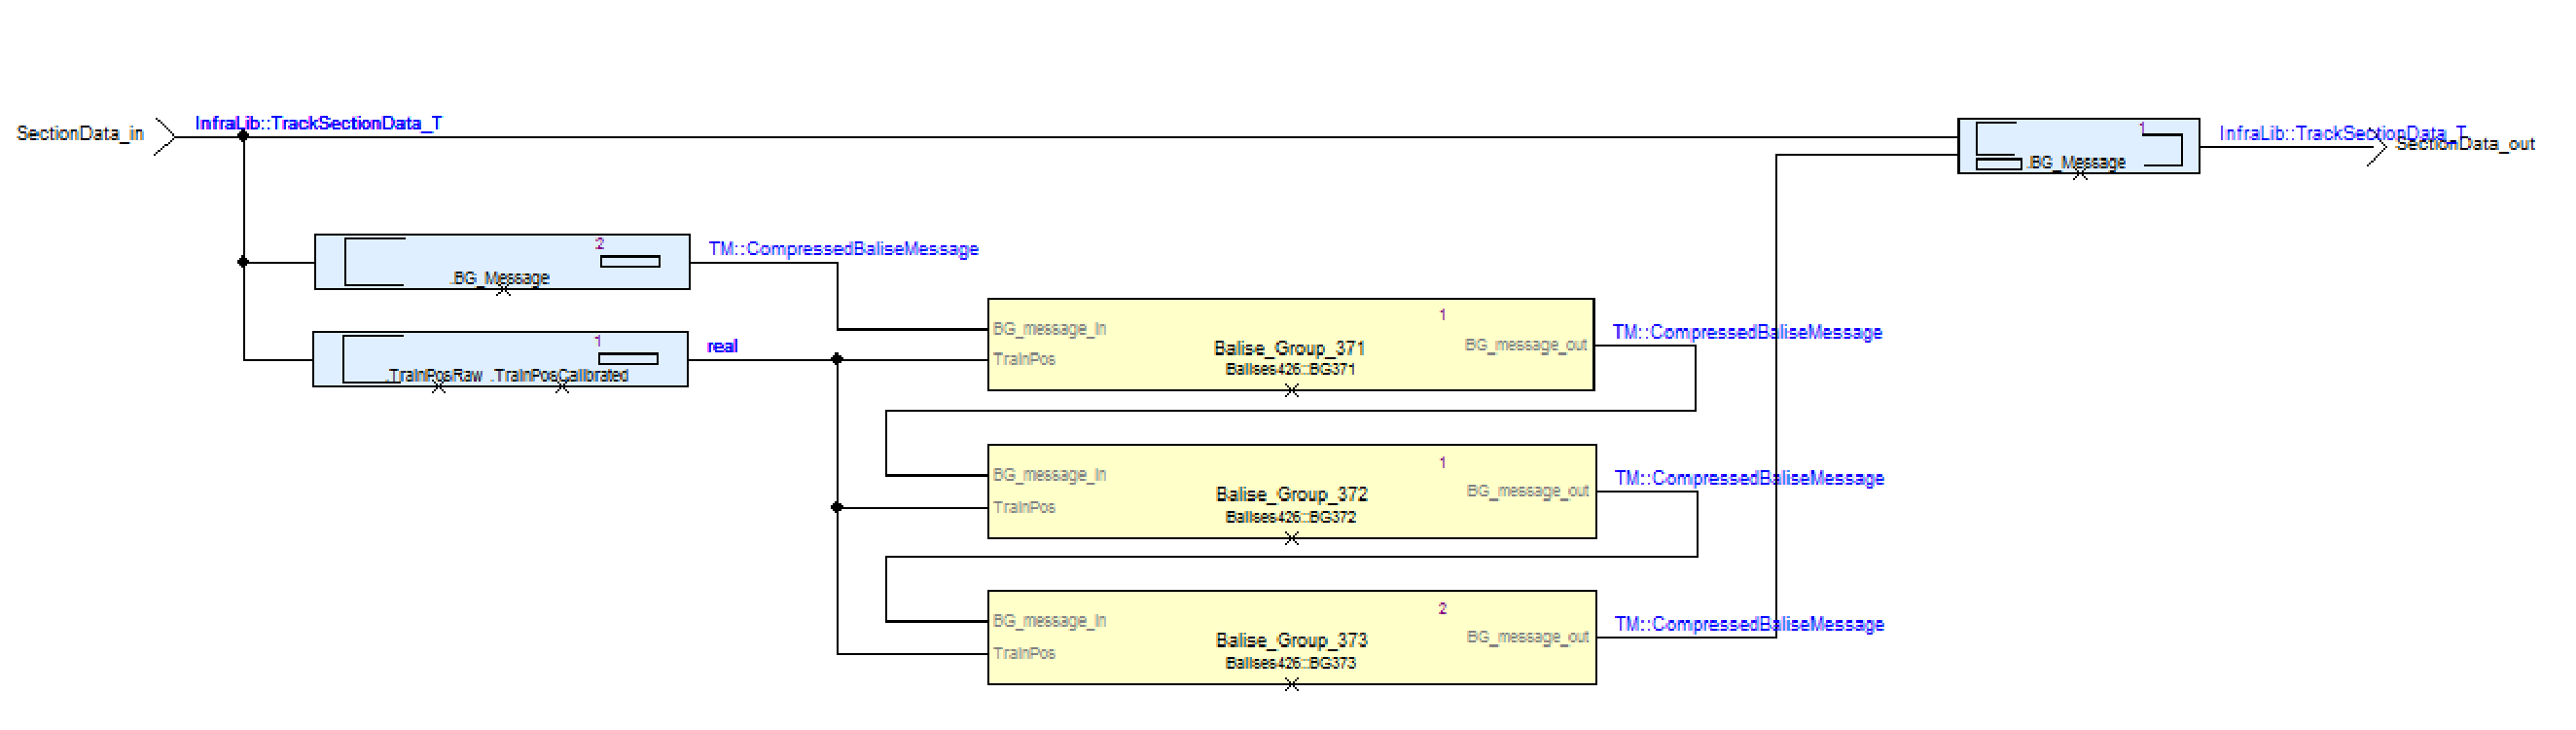
\includegraphics[angle=90, origin=c,width=2.5in]{images/DaisyChain.eps}
  \caption{Daisy Chained Balise Groups}
  \label{fig:daisy}
\end{figure}

As we will see in detail, we have used the daisy chain pattern in order to provided a structured, hierarchical model. There are several layers of daisy chains, which can be concatenated:
\begin{enumerate}
 \item Tracks 
 \item Sections (Sheets)
 \item Balise Groups
\end{enumerate}
Tracks, Sections and Balise Groups share the same semantics and interfaces and can be concatenated between each other.\newline It is however recommended to maintain the hierarchical structure as in the reference track model when constructing new tracks.
If we go one hierarchy level down, there is a daisy chain of balises inside each balise group model.
This pattern is more rigid, and will be described in the relevant section where we will discuss \emph{design templates} in more detail.\newline
Inside each balise, there are again daisy- chained operators to build messages and packets. Again, these will be discussed in more detail in the design templates chapter.\newline\newline
Equally, the radio message model is built using the same design principles.


\subsection{Where to find the information in the model}

The model is organised in SCADE packages. Each package contains specific elements or information.\newline

The main elements:

\begin{itemize}
 \item The Amsterdam Utrecht Reference Line: \textbf{AmsterdamUtrechtL2}\newline
 The track model is then hierarchically structured:
  \begin{itemize}
   \item Main balise model: \textbf{Amsterdam\_Utrecht\_Lijn1\_balises}\newline The balise model is grouped according to the Track Topology Sheets\newline (\textbf{SheetXX\_Name\_Balises}), which in turn contain the models for the balise groups, balises and for sending the  packets. 
   \item Main radio message model: \textbf{Amsterdam\_Utrecht\_Lijn1\_RBC}\newline The radio message model is grouped according to the Track Topology Sheets\newline (\textbf{SheetXX\_Name\_RBC}), which in turn contain the models for sending the messages and packets. 

  \end{itemize}
 \item The balise data for the Amsterdam- Utrecht Reference Line (NID\_C=426): \textbf{Balises426}.\newline \emph{The corrected balise positions are visible in the engineering data, as we have expressed them using SCADE constant expressions in the format OriginalPosition + Correction}
 \item The packet and message data for the Amsterdam- Utrecht Reference Line:  \textbf{Packets426} and \textbf{Messages\_426}, respectively.
 \item A packaging for the User Stories (with the original June 2015 milestone): \textbf{US\_Integration\_June}.
 \end {itemize}


There are some additional packages (that a normal user of the track model can ignore):
\begin{itemize}
 \item \textbf{FirstTest}: The first, short test track that was used to validate the concept
 \item \textbf{AmsterdamUtrechtL1}: A first version of the track model, containing Linking information sent from balise groups (That's why we called it "L1", for ETCS Level 1)
 \item \textbf{AmsterdamUtrechtL2\_original}: A version of the test track with balise positions (defined in \textbf{Balises426\_original} not aligned with the linking information
 \item \textbf{Internal\_Tests}: Some test routines that were used for user validation of the track model and the underlying libraries (such as TrackMessages)
 \item \textbf{Basics, Infra426}: internal definitions
\end{itemize} 

\subsection{Track model (balises)}

\begin{figure}[H]
  \centering
  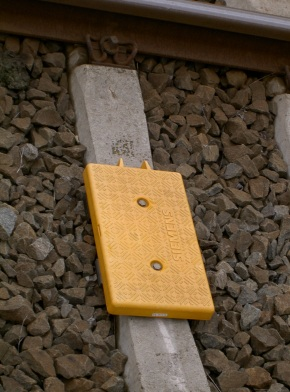
\includegraphics[width=2.5in]{images/Eurobalise.jpg}
  % picture by Francois Melchior, licensed under CC BY-SA 3.0
  \caption{Siemens Eurobalise}
  \label{fig:eurobalise}
\end{figure}

The track model provides the EVC kernel with a view of the balise infrastructure. The main functions of this model are:
\begin{itemize}
 \item When the train passes a balise group, it receives the telegrams of the balises, in the right sequence. The information is complete enough for the EVC to derive the BG's orientation and to position it using odometer data and, if applicable, linking information.
 \item When the train passes a balise, it receives the packets contained therein, if applicable. 
\end{itemize}

The main idea of the model is that it should dynamically react to a passing train. Instead of hard- wired scenarios, the simulated train can move forward, backwards, come to standstill and change speed, without any impact on the representation of the track in the simulation. The only determining factor for receiving balise information is whether or not the front end of the train is "close enough" to a balise in order to "see it".

\begin{figure}
  \centering
  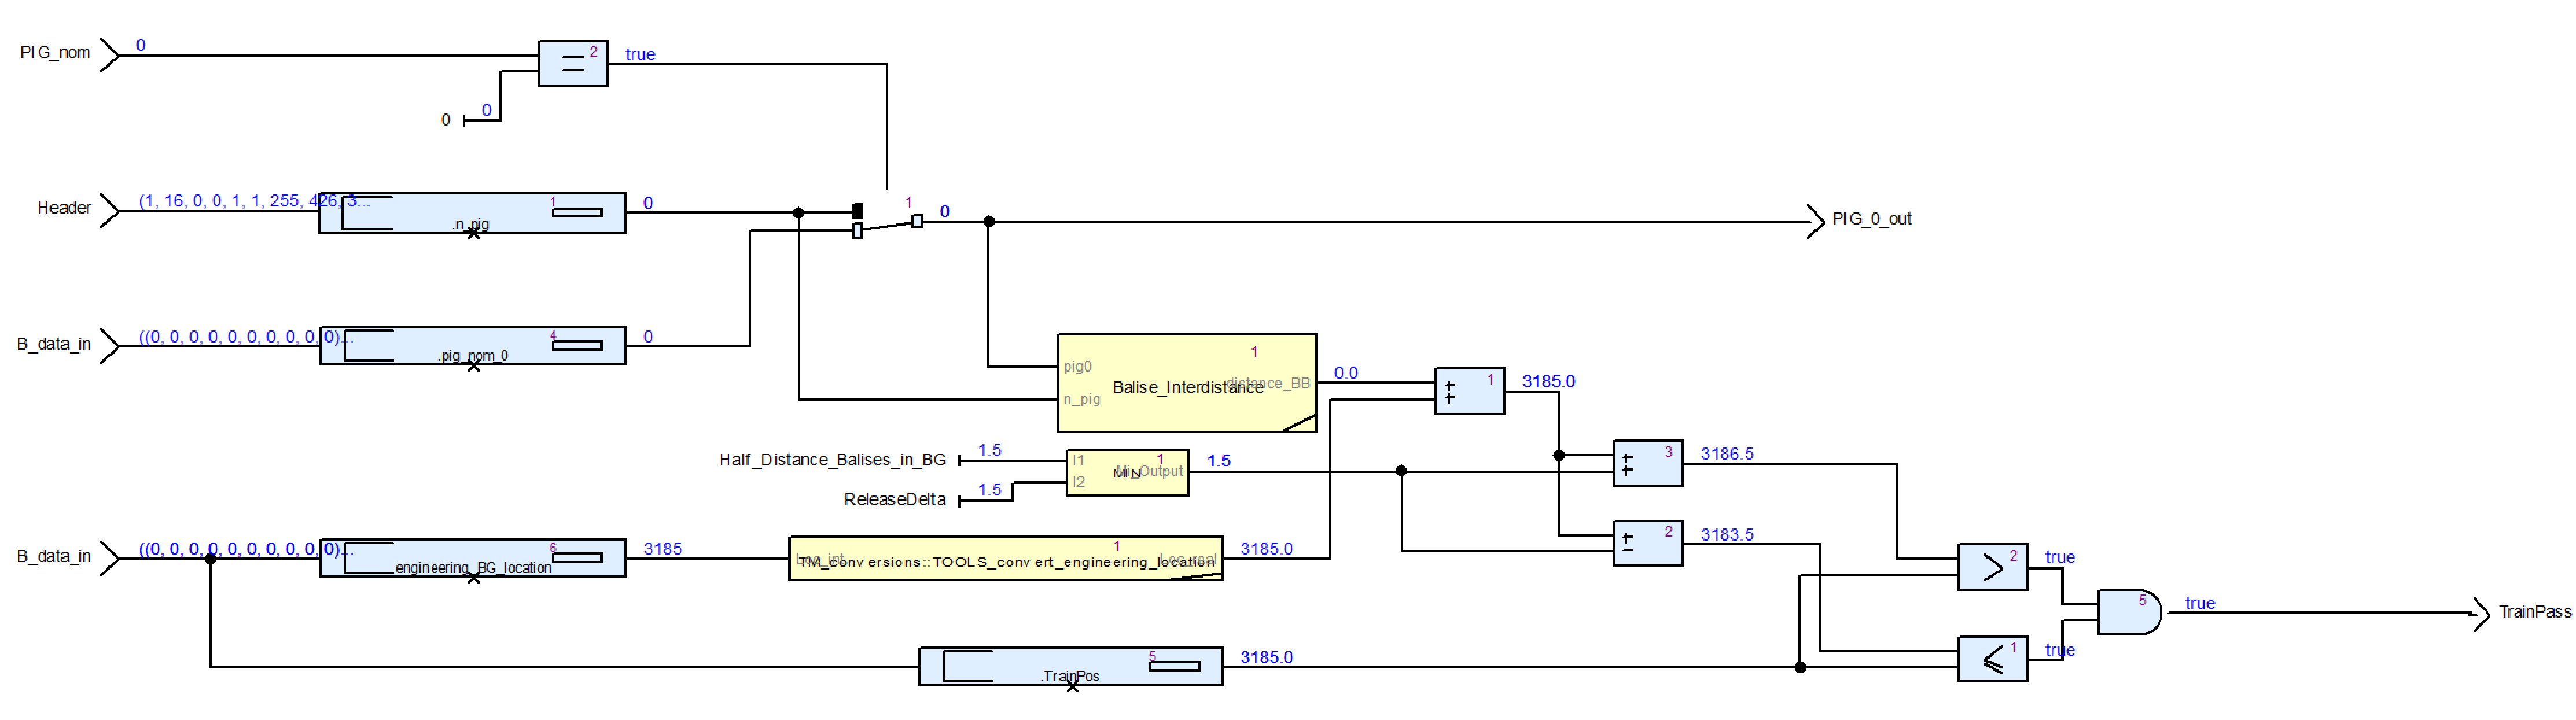
\includegraphics[angle=90, origin=c,width=2.5in]{images/TrainPass.eps}
  % picture by LEA Railergy, licensed under EUPL
  \caption{Triggering a Balise when the train is inside the defined distance bracket\newline (view from SCADE Suite Simulator)}
  \label{fig:balisepos}
\end{figure}

\subsubsection{Concept}

A real- world balise transmits its telegrams when a train passes. In our simulation, we try to model this as close as possible: As soon as a balise "sees" that a train is passing over it, it actively sends the information (telegram header and packets) through the daisy chain. At the end of the model, the resulting telegram and packets are transmitted to the simulated EVC. 
\begin{figure}[H]
  \centering
  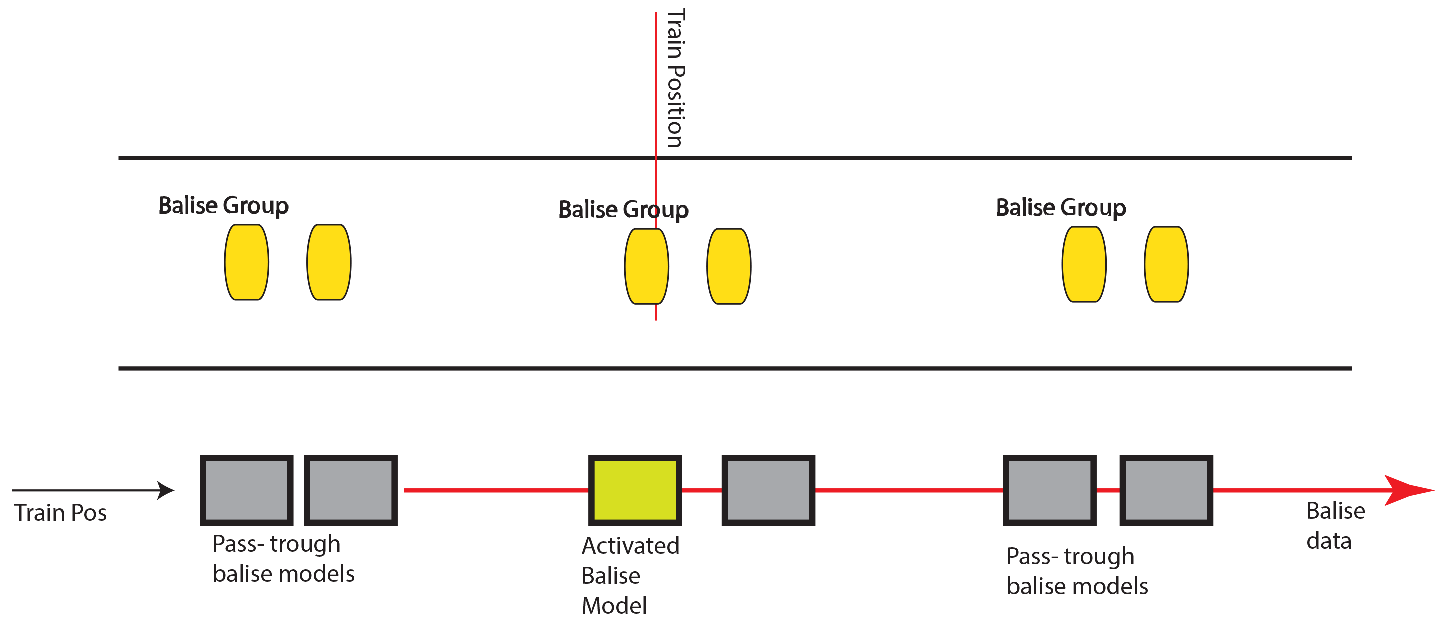
\includegraphics[width=6in]{images/BaliseChain.eps}
  % picture by LEA Railergy, licensed under EUPL
  \caption{Triggering a Balise in the Daisy Chain}
  \label{fig:balisechain}
\end{figure}



On model level we use the SCADE function \emph{InfraLib::Balise\_localisation} (see Figure \ref{fig:balisepos}), which checks whether the Balise is within a predefined distance bracket from the nominal train position.\newline\newline 
Note that this function takes into account the variable N\_PIG, which determines the position of a given balise ("I am the 1st") inside a balise group in order to determine the balise position. 




\subsubsection{The Balise Group Model}

\emph{We will not explain the models in full, but limit the discussion to the parts of the model that are track and data- specific. }

As the Amsterdam- Utrecht track is am ETCS Version 2.3.0 Level 2 track, we only see balise groups with 2 balises per group.
We present BG354. The relevant (corrected) engineering data are as follows:

\begin{table}[H]
  \centering
    \footnotesize\sffamily
\begin{tabular}{| l| l| l| r| l| l| l| l l}
\hline
\bf{NID\_C} & \bf{NID\_BG} & \bf{Lint} & \bf{km} & \bf{Or BG} & \bf{Or Line} & \bf{Line no} \\ 
\hline

426 & 354 & Asd-Zvg & 3185 & Utrecht & Z & spoor UB \\

\hline
\end{tabular}
\caption{Engineering data for BG354}
  \label{tab:bg354}
\end{table}

In the SCADE model, these data are defined as a \emph{constant expression}:
\begin{figure}[H]
  \centering
  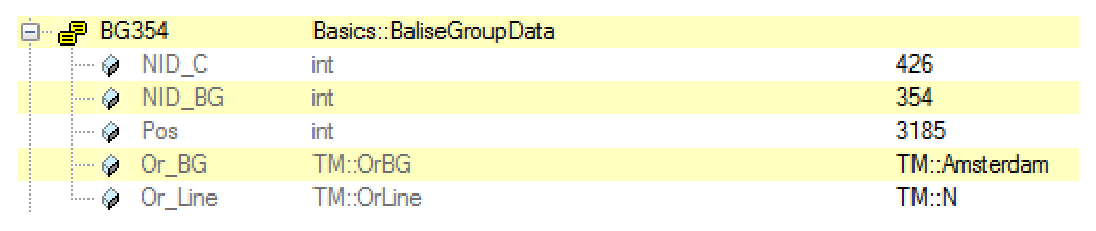
\includegraphics[width=4in]{images/EngDataBG354SCADE.eps}
  % picture by LEA Railergy, licensed under EUPL
  \caption{Engineering data for BG354 (view from SCADE model)}
  \label{fig:baliseposSCADE}
\end{figure}

\begin{figure}[H]
  \centering
  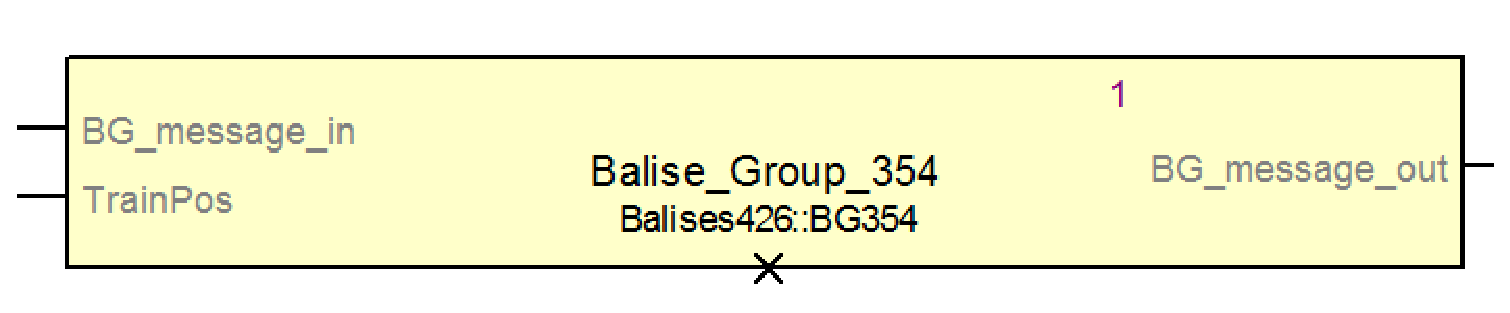
\includegraphics[width=4in]{images/BG354.eps}
  % picture by LEA Railergy, licensed under EUPL
  \caption{Interface and parameter reference for BG354 (view from SCADE model)}
  \label{fig:BG354SCADE}
\end{figure}

Figure \ref{fig:BG354SCADE} shows an external view of the operator implementing BG354.\newline
The interface is defined as follows:
\begin{itemize}
 \item input \textbf{BG\_message\_in}: data from daisy- chained BGs before
 \item input \textbf{TrainPos}: Train Position from simulation environment
 \item parameter \footnote{defined as "Hidden Input" in SCADE} \textbf{Engineering\_Data}: static definition of engineering data (from Figure \ref{fig:baliseposSCADE})
 \item output \textbf{BG\_message\_out}: data to daisy- chained BGs after
\end{itemize}
Looking inside the model (see Fig. \ref{fig:balisesBG354SCADE}), we will find two balises: Balise\_354\_0 and Balise Balise\_354\_1. Again, the daisy- chain pattern has been used in order to allow for a flexible design pattern (in the chapter "Explaining the templates", we will see how to design BGs with a different balise count between 1 and 8).\newline
The most important about this design pattern is that the ordering of the balises in a group is significant. If balise Balise\_354\_0 is the first in the chain and Balise\_354\_1 the second, then the passing train will see the BG as having nominal orientation. If the order is inverted, then the train will consider the BG to be oriented as reverse.

\begin{figure}[H]
  \centering
  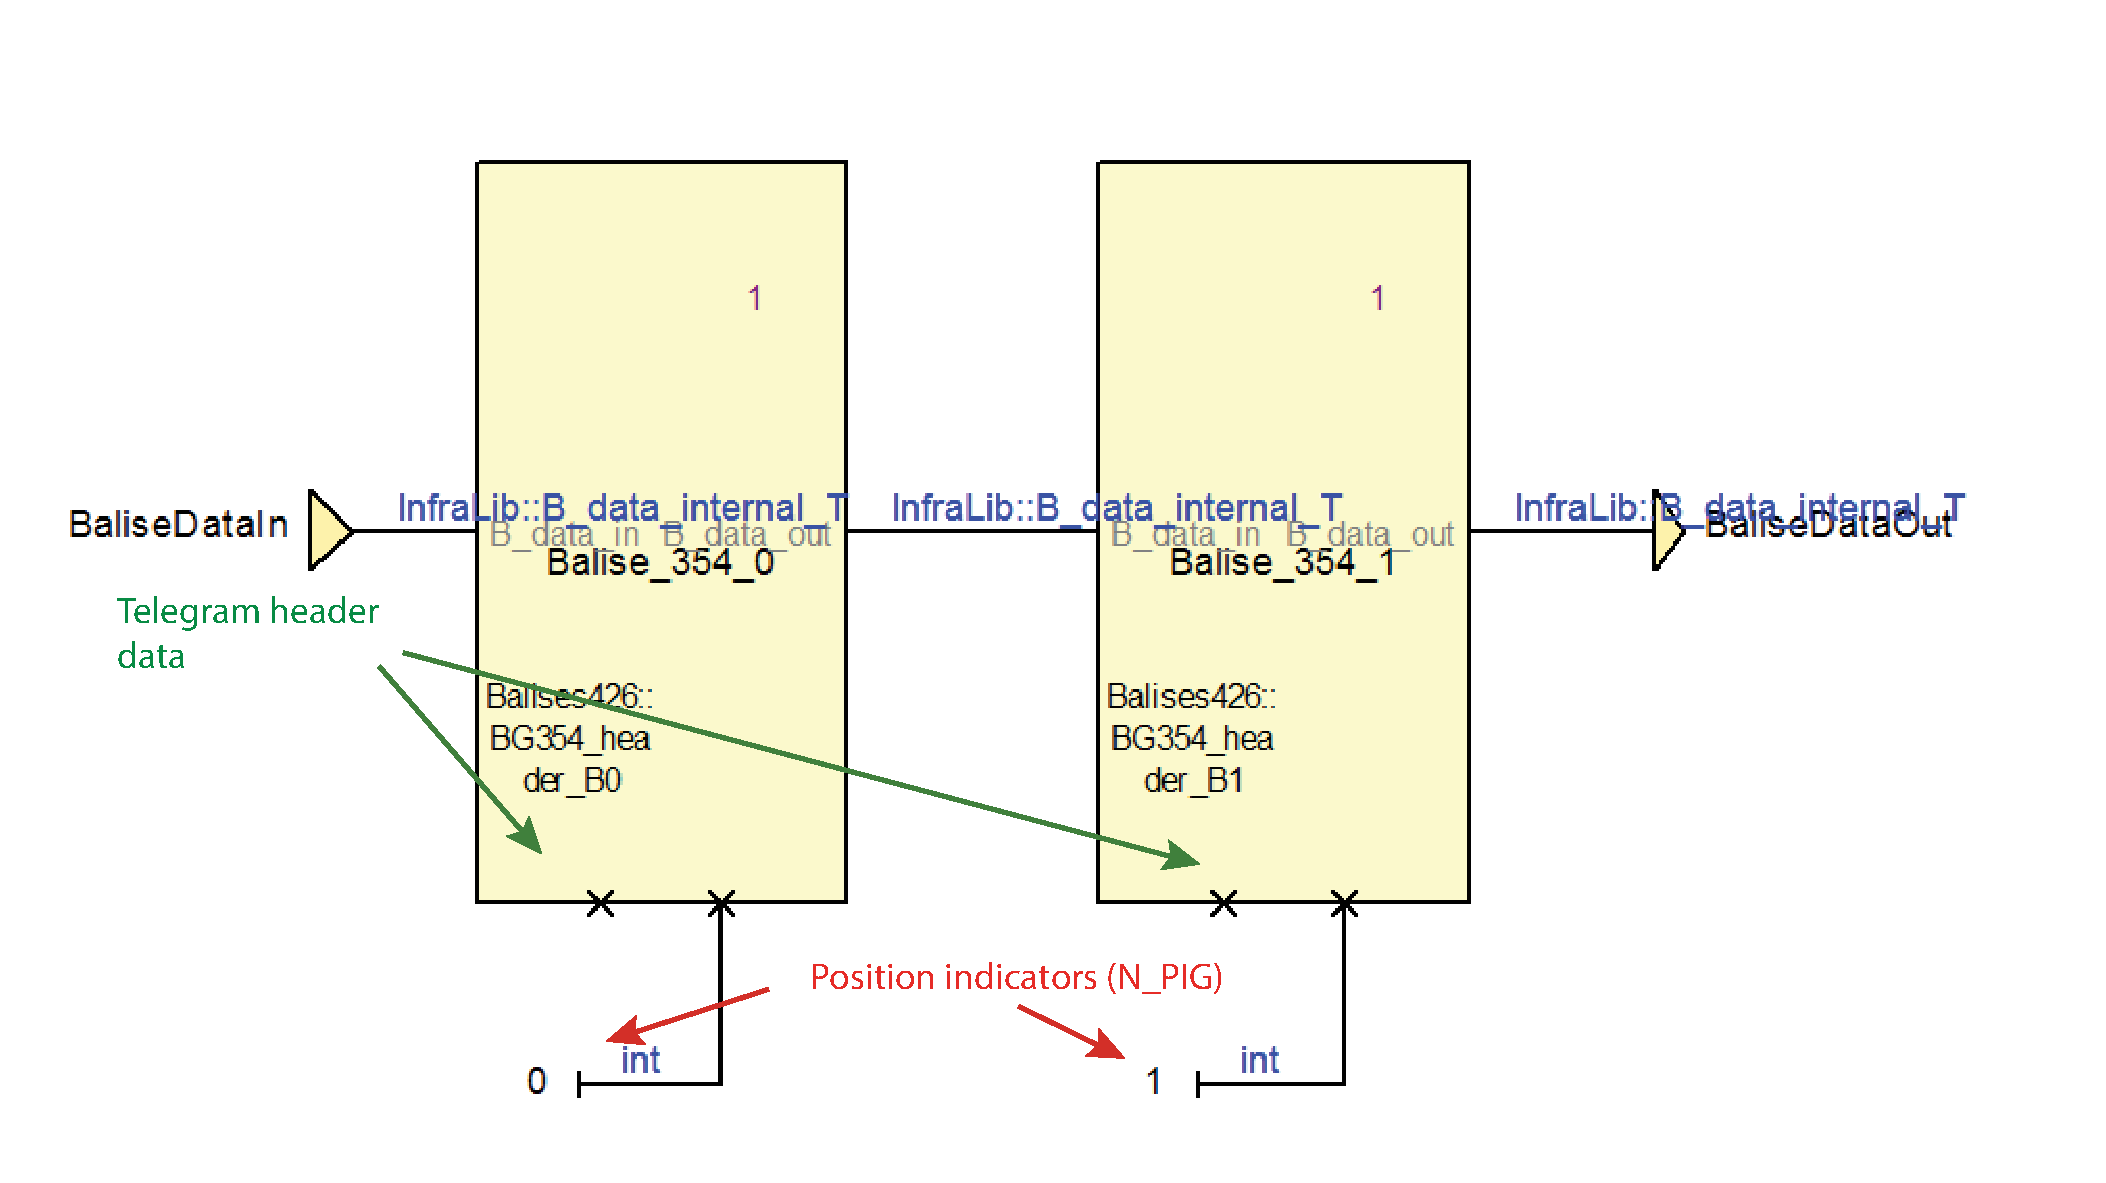
\includegraphics[width=5in]{images/BalisesInBG354.eps}
  % picture by LEA Railergy, licensed under EUPL
  \caption{Interface and parameter reference for balises in BG354 (view from SCADE model)}
  \label{fig:balisesBG354SCADE}
\end{figure}

The \emph{position indicators} are a fixed part of the design pattern. They must not be altered, and their order and position is fixed. The \emph{telegram header data} are used to generate the telegram headers sent to the EVC in case a train "passes" the balise, and also to calculate the balise position with reference to the engineering data. This means that the balise with the parameter N\_PIG=0 will release its telegram when the train passes the nominal position of the BG, while for balises with a different N\_PIG an offset will be used. The offset is also correctly calculated for reverse BGs.\newline
The orientation of the BG is determined by the N\_PIG information in the \emph{telegram header data}. If N\_PIG of the balise that is connected to the \emph{position indicator 0} = 0, then the BG is considered to be in nominal orientation. (of course, a reversing train will encounter it as reverse).

\begin{figure}[H]
  \centering
  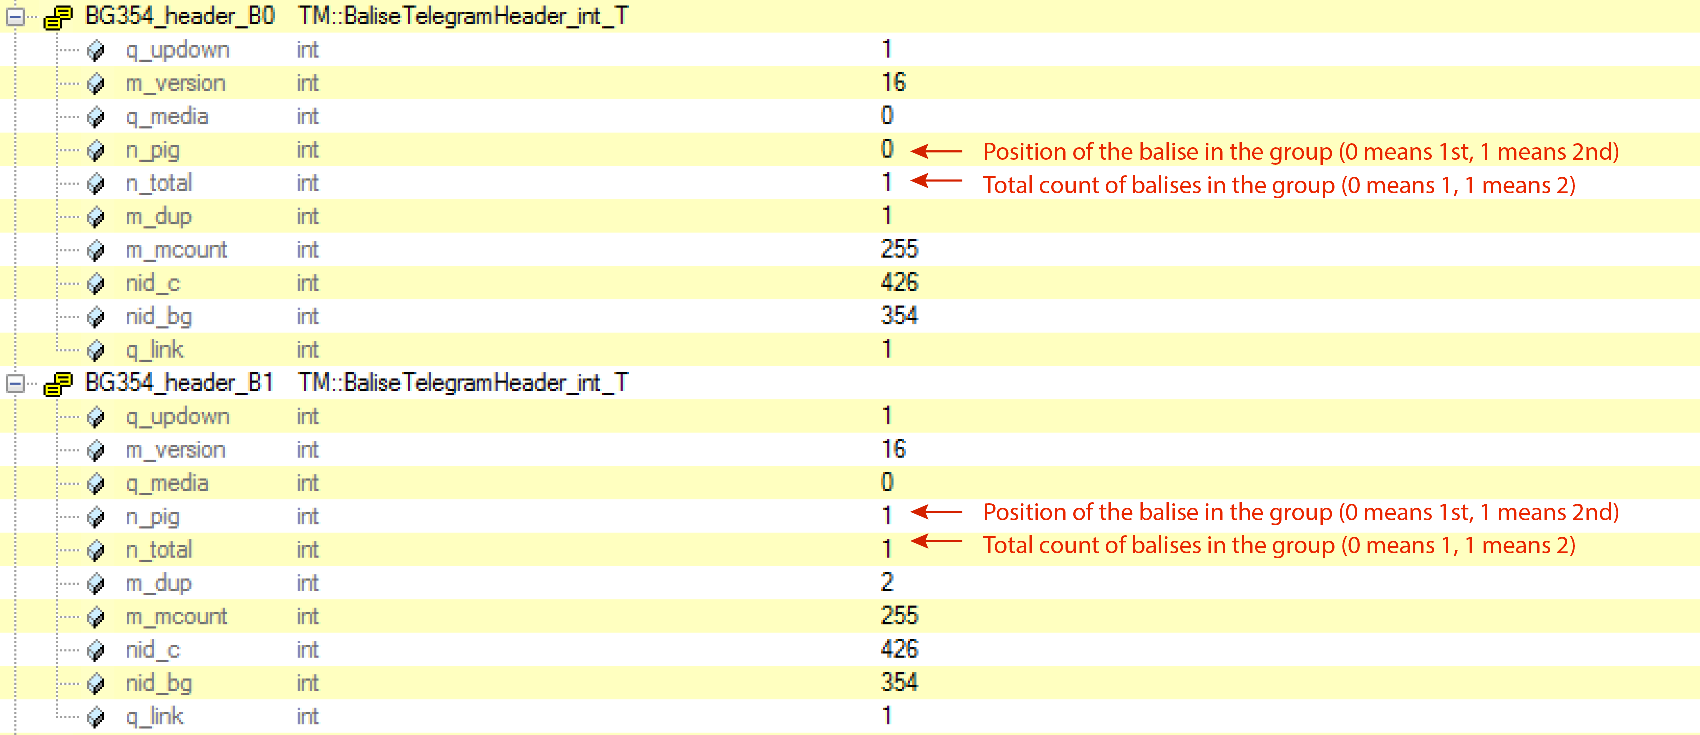
\includegraphics[width=6in]{images/Telegrams354.eps}
  % picture by LEA Railergy, licensed under EUPL
  \caption{Telegram data of BG354 (view from SCADE model)}
  \label{fig:telegrams354SCADE}
\end{figure}

Since the parameter n\_pig in the constant expression BG354\_header\_B0 is connected to the balise model with the position indicator 0, it is considered to be the 1st balise of a group in nominal orientation. 


\subsubsection{Sending balise telegrams and packets}

Again, the daisy- chain design pattern is being used.
While the telegram headers are sent by using internal logic in the balise model itself, a more elaborated design schema is used to send the packets that may be contained in a balise.

Comparing the packet data as found in the JRU log, we can see that the ordering of the send-packet operators in the balise is similar. This means that also the telegram will contain the packets in the same order as found in the JRU data.

The packet- specific send operators can be freely concatenated. They assure that all packets are merged into a message in a correct way. (For a deeper discussion of the underlying libraries, check the projects \textbf{BaliseLib.etp} and \textbf{TrackMessages.etp} that are part of the openETCS effort.)

\begin{table}[H]
  \footnotesize\sffamily
NID\_PACKET(8bits) = Session Management(42) \\
Q\_DIR(2bits) = Nominal(1) \\
L\_PACKET(13bits) = 113bits(113) \\
Q\_RBC(1bits) = Establish communication session(1) \\
NID\_C(10bits) = 426 \\
NID\_RBC(14bits) = 1(1) \\
    NID\_RADIO = Anonymous(lenght is more than 32bits or variable) \\
Q\_SLEEPSESSION(1bits) = Ignore session management information(0)" \\
\\
NID\_PACKET(8bits) = Conditional Level Transition Order(46) \\
Q\_DIR(2bits) = Nominal(1) \\
L\_PACKET(13bits) = 42bits(42) \\
M\_LEVELTR(3bits) = Level STM(1) \\
    NID\_STM(8bits) = ATB \\
N\_ITER(5bits) = 1(1) \\
    1: M\_LEVELTR[1](3bits) = Level 2(3)" \\
    \\
NID\_PACKET(8bits) = Conditional Level Transition Order(46) \\
Q\_DIR(2bits) = Reverse(0) \\
L\_PACKET(13bits) = 39bits(39) \\
M\_LEVELTR(3bits) = Level STM(1) \\
    NID\_STM(8bits) = ATB \\
N\_ITER(5bits) = 0(0)" \\
\\
NID\_PACKET(8bits) = National Values(3) \\
Q\_DIR(2bits) = Nominal(1) \\
L\_PACKET(13bits) = 186bits(186) \\
Q\_SCALE(2bits) = 1m(1) \\
D\_VALIDNV(15bits) = 0.0m(0) \\
N\_ITER(5bits) = 1(1) \\
    1: NID\_C[1](10bits) = 426 \\
V\_NVSHUNT(7bits) = 40km/h(8) \\
V\_NVSTFF(7bits) = 40km/h(8) \\
V\_NVONSIGHT(7bits) = 40km/h(8) \\
V\_NVUNFIT(7bits) = 10km/h(2) \\
V\_NVREL(7bits) = 15km/h(3) \\
D\_NVROLL(15bits) = 5.0m(5) \\
Q\_NVSRBKTRG(1bits) = No(0) \\
Q\_NVEMRRLS(1bits) = Release only at standstill possible(0) \\
V\_NVALLOWOVTRP(7bits) = 0km/h(0) \\
V\_NVSUPOVTRP(7bits) = 40km/h(8) \\
D\_NVOVTRP(15bits) = 200.0m(200) \\
T\_NVOVTRP(8bits) = 60s(60) \\
D\_NVPOTRP(15bits) = 60.0m(60) \\
M\_NVCONTACT(2bits) = Train trip(0) \\
T\_NVCONTACT(8bits) = 35s(35) \\
M\_NVDERUN(1bits) = Yes(1) \\
D\_NVSTFF(15bits) = Infinity(32767) \\
Q\_NVDRIVER\_ADHES(1bits) = Allowed(1)" \\
\\
NID\_PACKET(8bits) = End of information(255)" \\
\caption{Packets sent from BG354 as found in the JRU log}
  \label{tab:pbg354}
\end{table}

\begin{figure}[H]
  \centering
  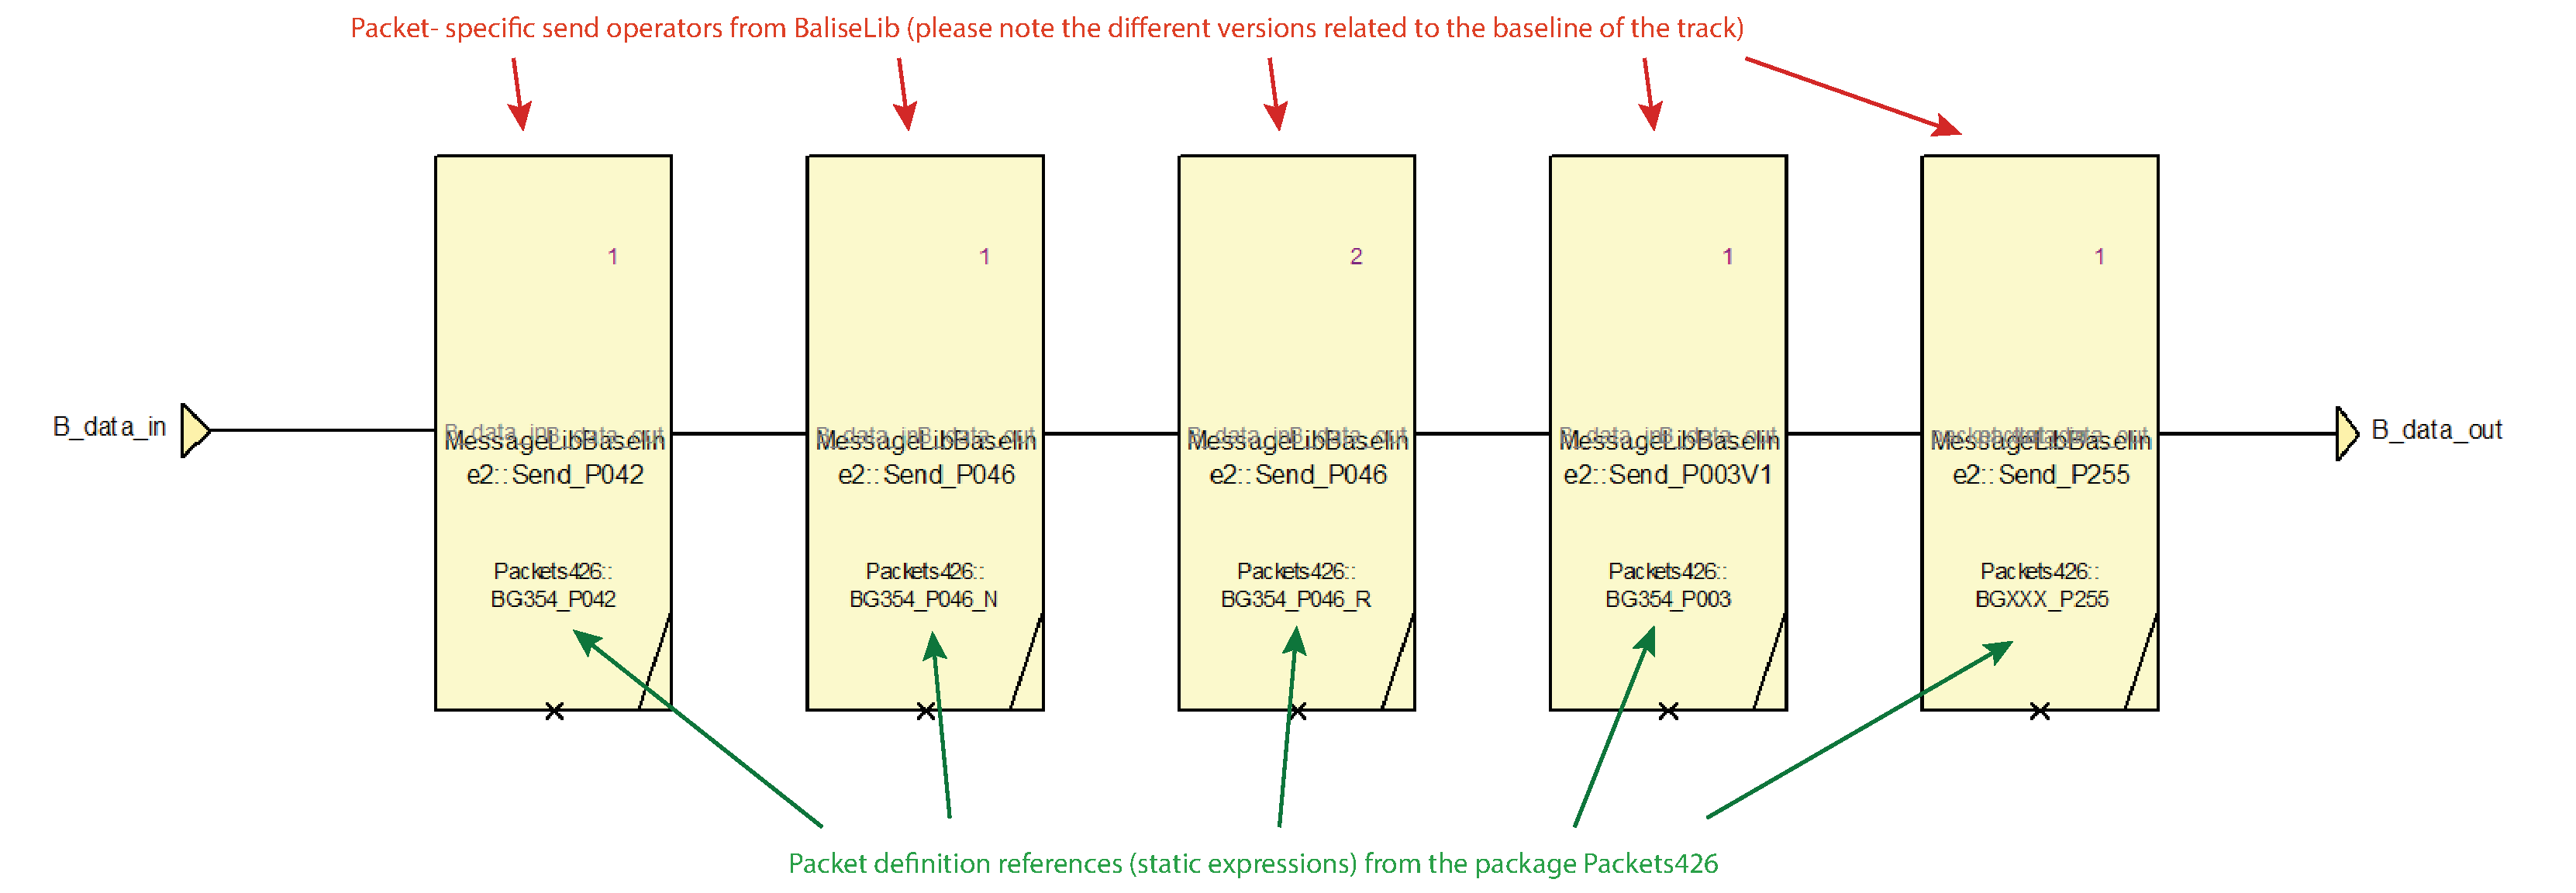
\includegraphics[width=6.5in]{images/PacketsBG354.eps}
  % picture by LEA Railergy, licensed under EUPL
  \caption{Sending packets from BG354 (view from SCADE model)}
  \label{fig:packets354SCADE}
\end{figure}

\emph{(Note: The packet definitions for BG354 in the SCADE model can be found in Packets426::BG354\_Pxxx)}

\subsubsection{Driving the train: Train Position vs. Balise Position}

Looking at the track topology maps, we can see that the engineering positions of balise groups that a train may pass can be on different track sections that may exhibit different origins for the distances (kilometres). These different coordinate systems are of course also reflected in the engineering data.

\begin{figure}[H]
  \centering
  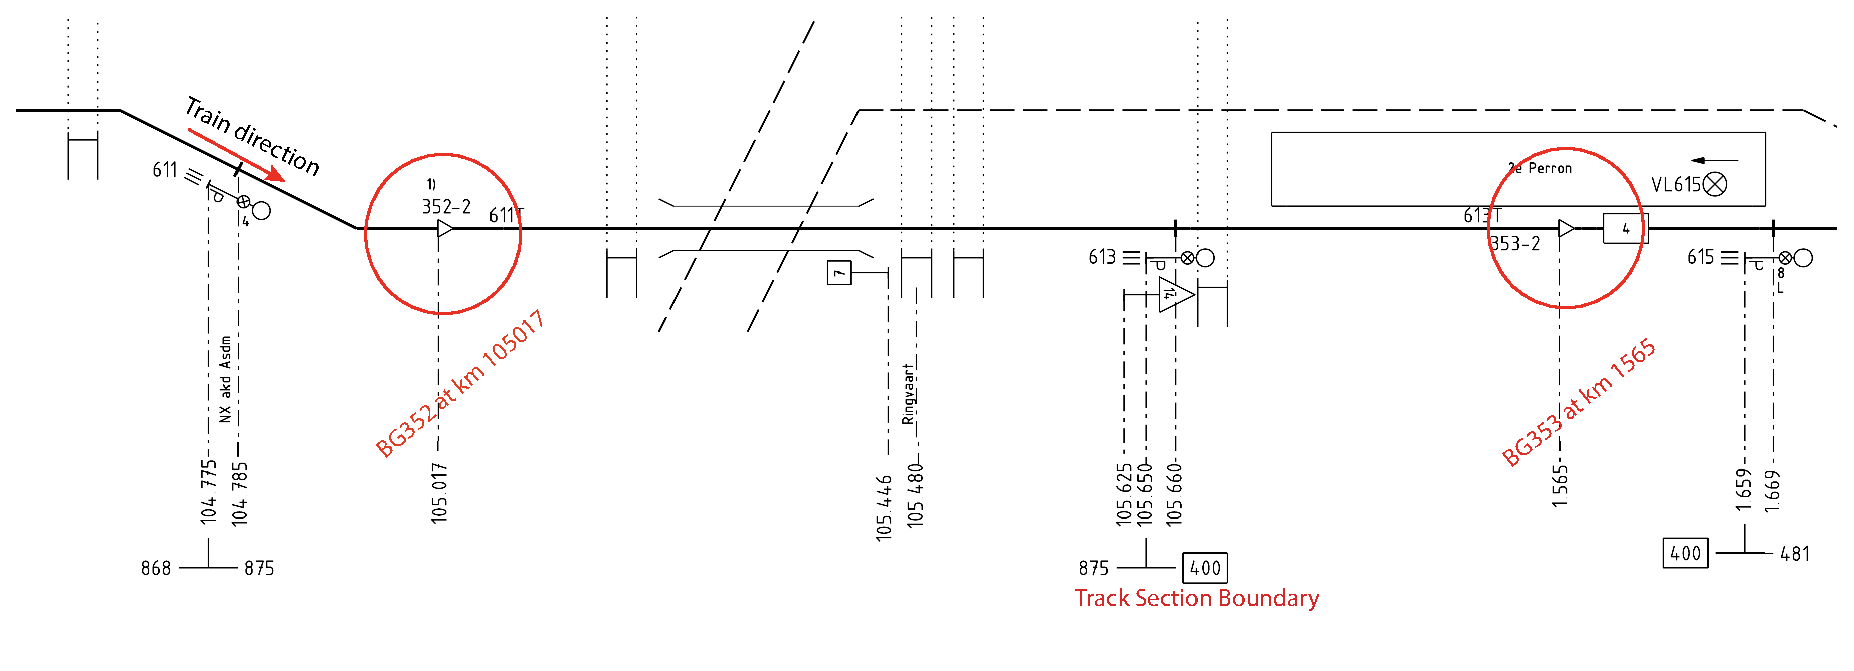
\includegraphics[width=6in]{images/CoordJump.eps}
   \caption{Balises in different local coordinate systems (depending on track sections)}
  \label{fig:balisecoord}
\end{figure}

Our train "knows nothing" about those coordinate systems: It starts at position 0 and while it drives on, the train position increases steadily when the train moves forward, and decreases when it moves backwards.\newline
On the other hand, the balises will only emit their telegrams when they see that the train position equals their own location (see figure \ref{fig:balisepos}).\newline
We therefore need a method to position the train correctly inside the track sections.

\begin{figure}[H]
  \centering
  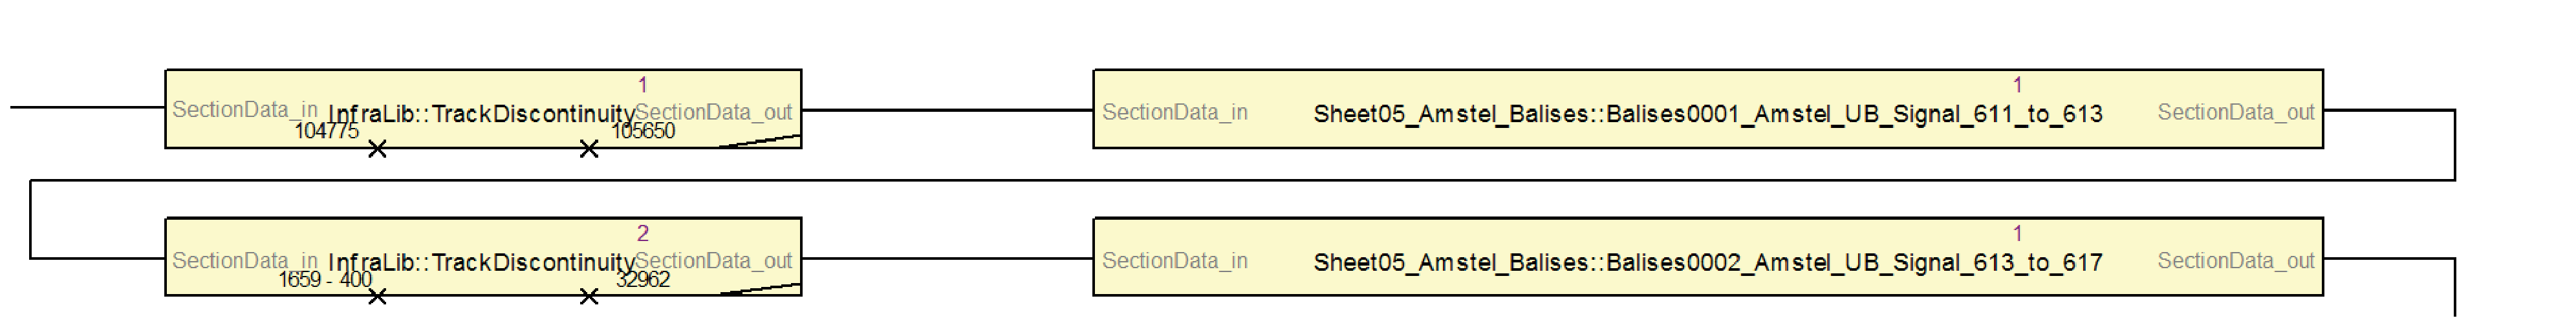
\includegraphics[width=6.5in]{images/TrackDiscont.eps}
   \caption{Track Discontinuity modelling (view from SCADE model)}
  \label{fig:trackjump}
\end{figure}

The operator InfraLib::TrackDiscontinuity takes two parameters:
\begin{itemize}
 \item \emph{StartSection}: kilometre at the start of the track section
 \item \emph{EndSection}: kilometre at the end of the track section
\end{itemize}
When placed in the daisy chain \emph{before} the concerned track section, the balises inside this section will see the simulated train in their local coordinate system. Track sections with such discontinuities can be concatenated. Each section will see the train in its local coordinate system.\newline\newline
When comparing the model with the track layout plan, we can observe that the section in the Scade Operator  \emph{Balises0001\_Amstel\_UB\_Signal\_611\_to\_613} are between km 104775 and km 105650, which is between signal 611 and signal 613.\newline\newline
For the section in the Scade Operator  \emph{Balises0001\_Amstel\_UB\_Signal\_613\_to\_617}, we had to define the beginning of the section to start also at signal 613. As there is no absolute kilometre value describing the position of this signal in the coordinate system of the following track, we have simply defined a constant expression to define the parameter \emph{StartSection} by using the available distance information between signal 613 and BG353. The \emph{EndSection} parameter is the latest position known from the User Story definition and is in fact located at Utrecht CS.

\subsection{Radio Message simulation}

The basic design principles used for the balise model (daisy chaining, merging of packets into a compressed format) apply also for the radio message model.\newline
The main differences are:
\begin{itemize}
 \item While balises contain a telegram header which always contains the same set of information, plus a set of packets (at least a packet 255), radio messages are composed of a Message (as defined in Subset-026 chapter 8 \cite{SRS026-8}) plus optional packets. 
 \item The balise model activates a balise when a train passes, while the radio message model expects an external trigger signal which comes from the RBC model.
\end{itemize}

\subsubsection{Base data for the radio message model}
The only available source of information for the creation of the radio message simulation model are the data logged in the JRU files provided as part of the User Story definitions.\newline
As part of our analysis work, we have created a cross- reference table for the simulated radio messages.\newline
The columns must be read as follows:
\begin{enumerate}
 \item \textbf{NID\_MESSAGE}: Message (as defined in Subset-026 chapter 8 \cite{SRS026-8}).\newline The messages are defined as constant expressions in the package \emph{Messages\_426} and named using the format LRBG\_\textbf{nn.}\_D\_\textbf{ddddd}\_\textbf{f}\_M\textbf{mmm} with:
	\begin{itemize}
	 \item \textbf{nnn} = NID\_BG value of NID\_LRBG (the NID\_C value is assumed to be 426, as already expressed in the package name)
	 \item \textbf{ddddd} = the integer part of the distance from the LRBG where the radio message was recorded, in meters. The number is padded with leading zeroes if less the 5 significant digits exist.
	 \item \textbf{f} = the fractional part of the distance from the LRBG where the radio message was recorded, in tenths of meters.
	 \item \textbf{mmm} = the NID\_MESSAGE. Padded with leading zeroes if less then 3 significant digits exist.
	\end{itemize}
 \item \textbf{Packets}: Optional packets, as defined in Subset-026 chapter 8 \cite{SRS026-8} and described in detail in Subset-026 chapters 7 \cite{SRS026-7} and, where applicable in chapter 6 \cite{SRS026-6}.\newline The packet definitions in the form of SCADE constant expressions can be found in the package \emph{Packets426}. 
 \item \textbf{Trigger}: Integer value. The radio message simulation model observers the input \emph{Trigger} which is propagated through all Send Radio Message operators that are daisy- chained to form the simulation model. If an operator receives a trigger value corresponding to its local trigger parameter definition, it will release the message and all optional packets it contains and forward them through the daisy chain to the EVC. The trigger has, by convention, the format nnndddddf with:
\begin{itemize}
	 \item \textbf{nnn} = NID\_BG value of NID\_LRBG (the NID\_C value is assumed to be 426, as already expressed in the package name)
	 \item \textbf{ddddd} = the integer part of the distance from the LRBG where the radio message was recorded, in meters. The number is padded with leading zeroes if less the 5 significant digits exist.
	 \item \textbf{f} = the fractional part of the distance from the LRBG where the radio message was recorded, in tenths of meters.
	 	\end{itemize}
 \item \textbf{LRBG}: NID\_BG value of NID\_LRBG (the NID\_C value is assumed to be 426).\newline\newline \emph{Important note: This value refers to the LRBG known to the train at the reception of the message. It may differ from the LRBG which is referenced in the message itself!}
 \item \textbf{Distance}: Distance from the LRBG at which the message was received according to the JRU data, in meters, resolution 0,1m
\end{enumerate}

\begin{longtable}{|l |l |l |l |r |}
\hline
\textbf{NID\_MESSAGE} & \textbf{Packets} & \textbf{Trigger} & \textbf{LRBG} & \textbf{Distance} \\
\hline
\endfirsthead
\hline
NID\_MESSAGE & Packets & Trigger & LRBG & Distance \\
\hline
\endhead
\hline
\multicolumn{5}{r}{{Continued next page\ldots}} \
\endfoot
\hline
\caption{Cross reference table for the radio messages relevant for the Proof of Concept,\newline partial list covering the sheets Amstel and Bijlmer}
  \label{tab:xrefradio}
\endlastfoot

32 & None & 353003192 & 353 & 319.2 \\
8 & None & 353004219 & 353 & 421.9 \\
24 & P57 & 353004310 & 353 & 431.0 \\
24 & None & 353004413 & 353 & 441.3 \\
24 & None & 353004972 & 353 & 497.2 \\
24 & None & 353006561 & 353 & 656.1 \\
24 & None & 353008532 & 353 & 853.2 \\
24 & None & 353010375 & 353 & 1037.5 \\
24 & None & 353012387 & 353 & 1238.7 \\
24 & None & 353014483 & 353 & 1448.3 \\
24 & None & 354000537 & 354 & 53.7 \\
24 & None & 354000902 & 354 & 90.2 \\
3 & P15, P21, P27, P3, P5, P41, P65 & 354002753 & 354 & 275.3 \\
24 & None & 354004835 & 354 & 483.5 \\
24 & None & 354006798 & 354 & 679.8 \\
24 & None & 351000333 & 351 & 33.3 \\
3 & P15, P21, P27, P3, P5, P41, P65 & 351000549 & 351 & 54.9 \\
24 & None & 351000656 & 351 & 65.6 \\
24 & None & 351000723 & 351 & 72.3 \\
15 & None & 355000894 & 355 & 89.4 \\
24 & None & 355001262 & 355 & 126.2 \\
24 & None & 355001330 & 355 & 133.0 \\
15 & None & 356000485 & 356 & 48.5 \\
24 & None & 357000389 & 357 & 38.9 \\
24 & None & 357000591 & 357 & 59.1 \\
24 & None & 357001511 & 357 & 151.1 \\
24 & None & 358000540 & 358 & 54.0 \\
24 & None & 358000916 & 358 & 91.6 \\
15 & None & 358001231 & 358 & 123.1 \\
24 & None & 359000371 & 359 & 37.1 \\
24 & None & 359000500 & 359 & 50.0 \\
24 & None & 360000516 & 360 & 51.6 \\
24 & None & 360000980 & 360 & 98.0 \\
24 & None & 360001835 & 360 & 183.5 \\
24 & None & 360002492 & 360 & 249.2 \\
24 & None & 360002766 & 360 & 276.6 \\
24 & None & 360003507 & 360 & 350.7 \\
24 & None & 360004244 & 360 & 424.4 \\
24 & None & 361000278 & 361 & 27.8 \\
24 & None & 361000442 & 361 & 44.2 \\
24 & None & 362000298 & 362 & 29.8 \\
24 & None & 362000347 & 362 & 34.7 \\
24 & None & 362000769 & 362 & 76.9 \\
24 & None & 362001089 & 362 & 108.9 \\
15 & None & 362001249 & 362 & 124.9 \\
24 & None & 362001364 & 362 & 136.4 \\
24 & None & 362001588 & 362 & 158.8 \\
24 & None & 362001820 & 362 & 182.0 \\
24 & None & 362002166 & 362 & 216.6 \\
24 & None & 362002273 & 362 & 227.3 \\
24 & None & 362002606 & 362 & 230.6 \\
3 & P15, P21, P27, P3, P5, P41, P65 & 362002307 & 362 & 230.7 \\
3 & P15, P21, P27, P3, P5, P41, P65 & 362002389 & 362 & 238.9 \\
24 & None & 363000258 & 363 & 25.8 \\
24 & None & 364000173 & 364 & 17.3 \\
24 & None & 364000366 & 364 & 36.6 \\
3 & P15, P21, P27, P3, P5, P41, P65 & 364000911 & 364 & 91.1 \\
24 & None & 364001742 & 364 & 174.1 \\
24 & None & 365000582 & 365 & 58.2 \\
24 & None & 366000521 & 366 & 52.1 \\
24 & None & 367000154 & 367 & 15.4 \\
24 & None & 367000599 & 367 & 59.9 \\
24 & None & 367001513 & 367 & 151.3 \\
24 & None & 368000592 & 368 & 59.2 \\
24 & None & 369000733 & 369 & 73.3 \\
24 & None & 369001060 & 369 & 106.0 \\
15 & None & 369002313 & 369 & 231.3 \\
24 & None & 369002772 & 369 & 277.2 \\
24 & None & 369004516 & 369 & 451.6 \\
24 & None & 341000724 & 341 & 72.4 \\
15 & None & 341001344 & 341 & 134.4 \\
24 & None & 341001559 & 341 & 155.9 \\
24 & None & 341003500 & 341 & 350.0 \\

\end{longtable}


\emph{Remark: with the exception of the message received at LRBG=353 and the distance=431.0, General Messages (M024) are not part of this model, but are dynamically created inside the RBC model.}

\subsection{The radio message formal model}
\subsubsection{Concatenating operators}
As the design principles have already been discussed in the \emph{Balise Model} chapter of this text, we will mainly highlight the differences. Figure \ref{fig:rbcchain} shows an example of a send radio message model.
\begin{itemize}
 \item The name of the operators corresponds with the name of the message definition (for example LRBG\_353\_D\_00319\_2\_M032; see also the legend for table \ref{tab:xrefradio})
 \item At the hidden inputs we see the trigger value (for example 353003192)
\end{itemize}
 
\begin{figure}[H]
  \centering
  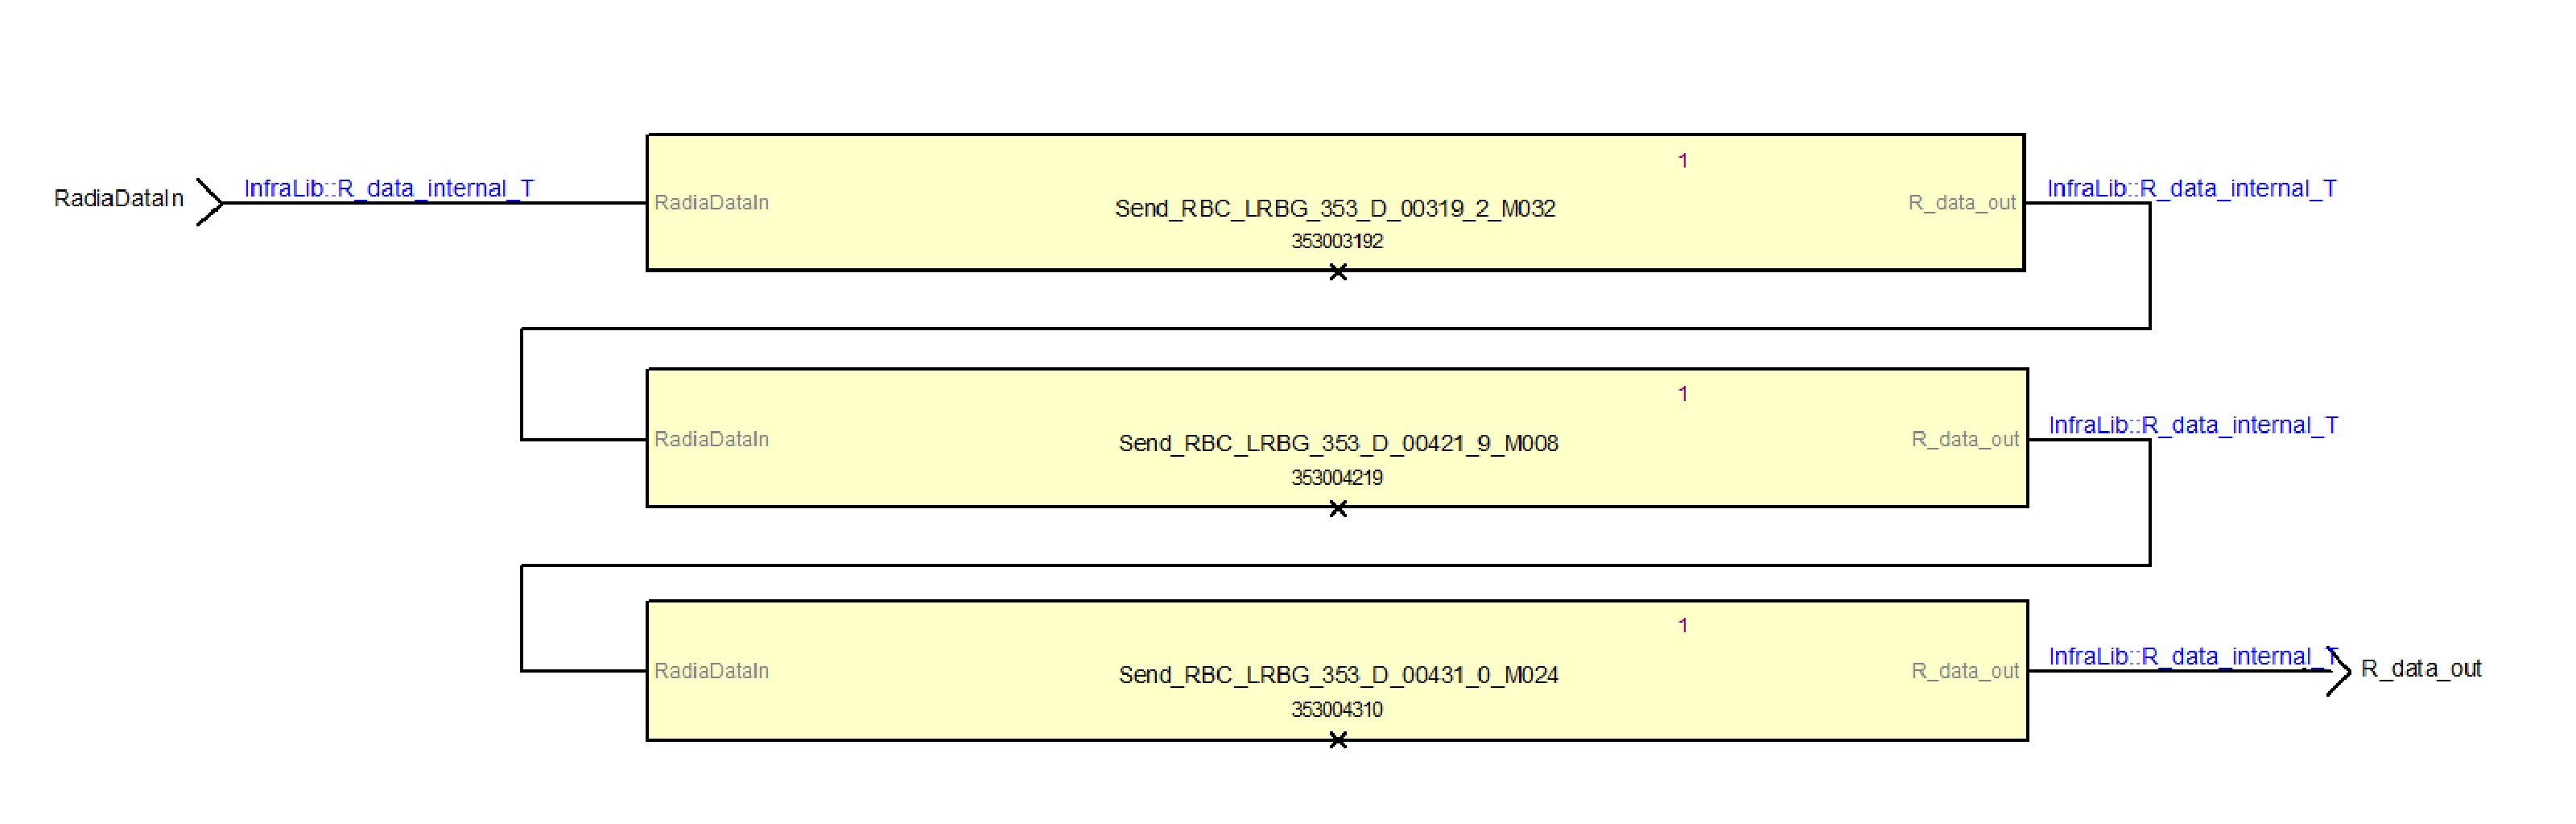
\includegraphics[width=6.5in]{images/rbcchain.eps}
   \caption{Daisy- chained Send Radio message operators (view from SCADE model)}
  \label{fig:rbcchain}
\end{figure}
\subsubsection{Activating the send function}
Going one level deeper inside the operator \emph{Send\_RBC\_LRBG\_353\_D\_00319\_2\_M032}, we see (figure \ref{fig:sendRM}) that:
\begin{itemize}
 \item If The trigger value received from RBC (via RadioDataIn) equals the parameter (via TriggerValue), then the function \emph{Build\_RBC\_Message\_LRBG\_353\_D\_00319\_2\_M032} is activated,
 \item Otherwise, the RadioDataIn value is just propagated to the output R\_data\_out.
\end{itemize}
\begin{figure}[H]
  \centering
  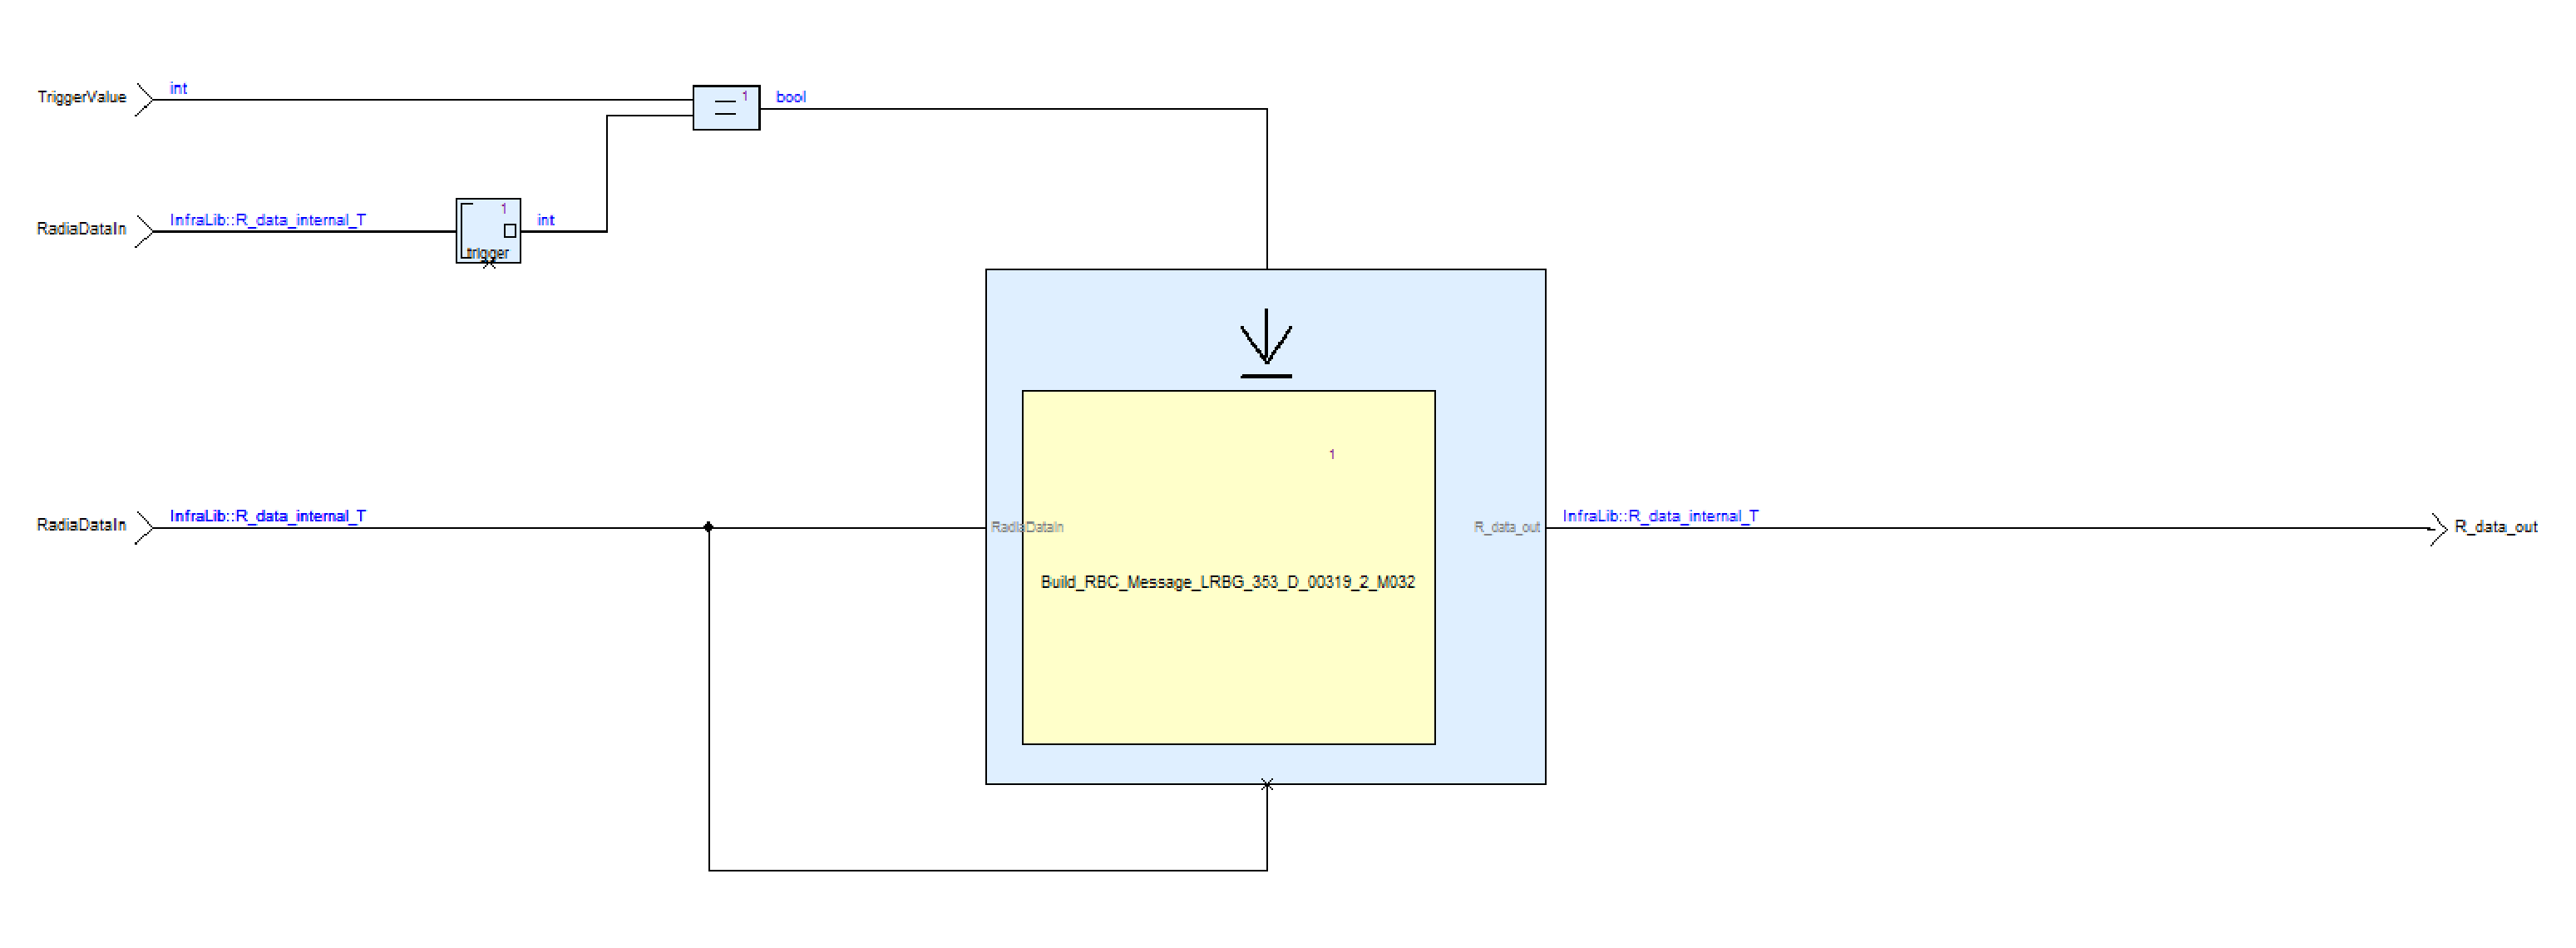
\includegraphics[width=6.5in]{images/sendRM.eps}
   \caption{Send Radio Message (view from SCADE model)}
  \label{fig:sendRM}
\end{figure}
This means that if the trigger is valid, the messages and packets defined in this operator will be merged to the data flow representing the radio messages. Otherwise, any other messages defined elsewhere will be passed along the daisy chain.\newline

\subsubsection{Merging information}

If the RBC commands that a message be sent, we have to merge the defined message and packet information onto the data flow that runs along the daisy chain. In our example in figure \ref{fig:composeRM}, a message 32 must be sent, which contains no optional packets.
\begin{figure}[H]
  \centering
  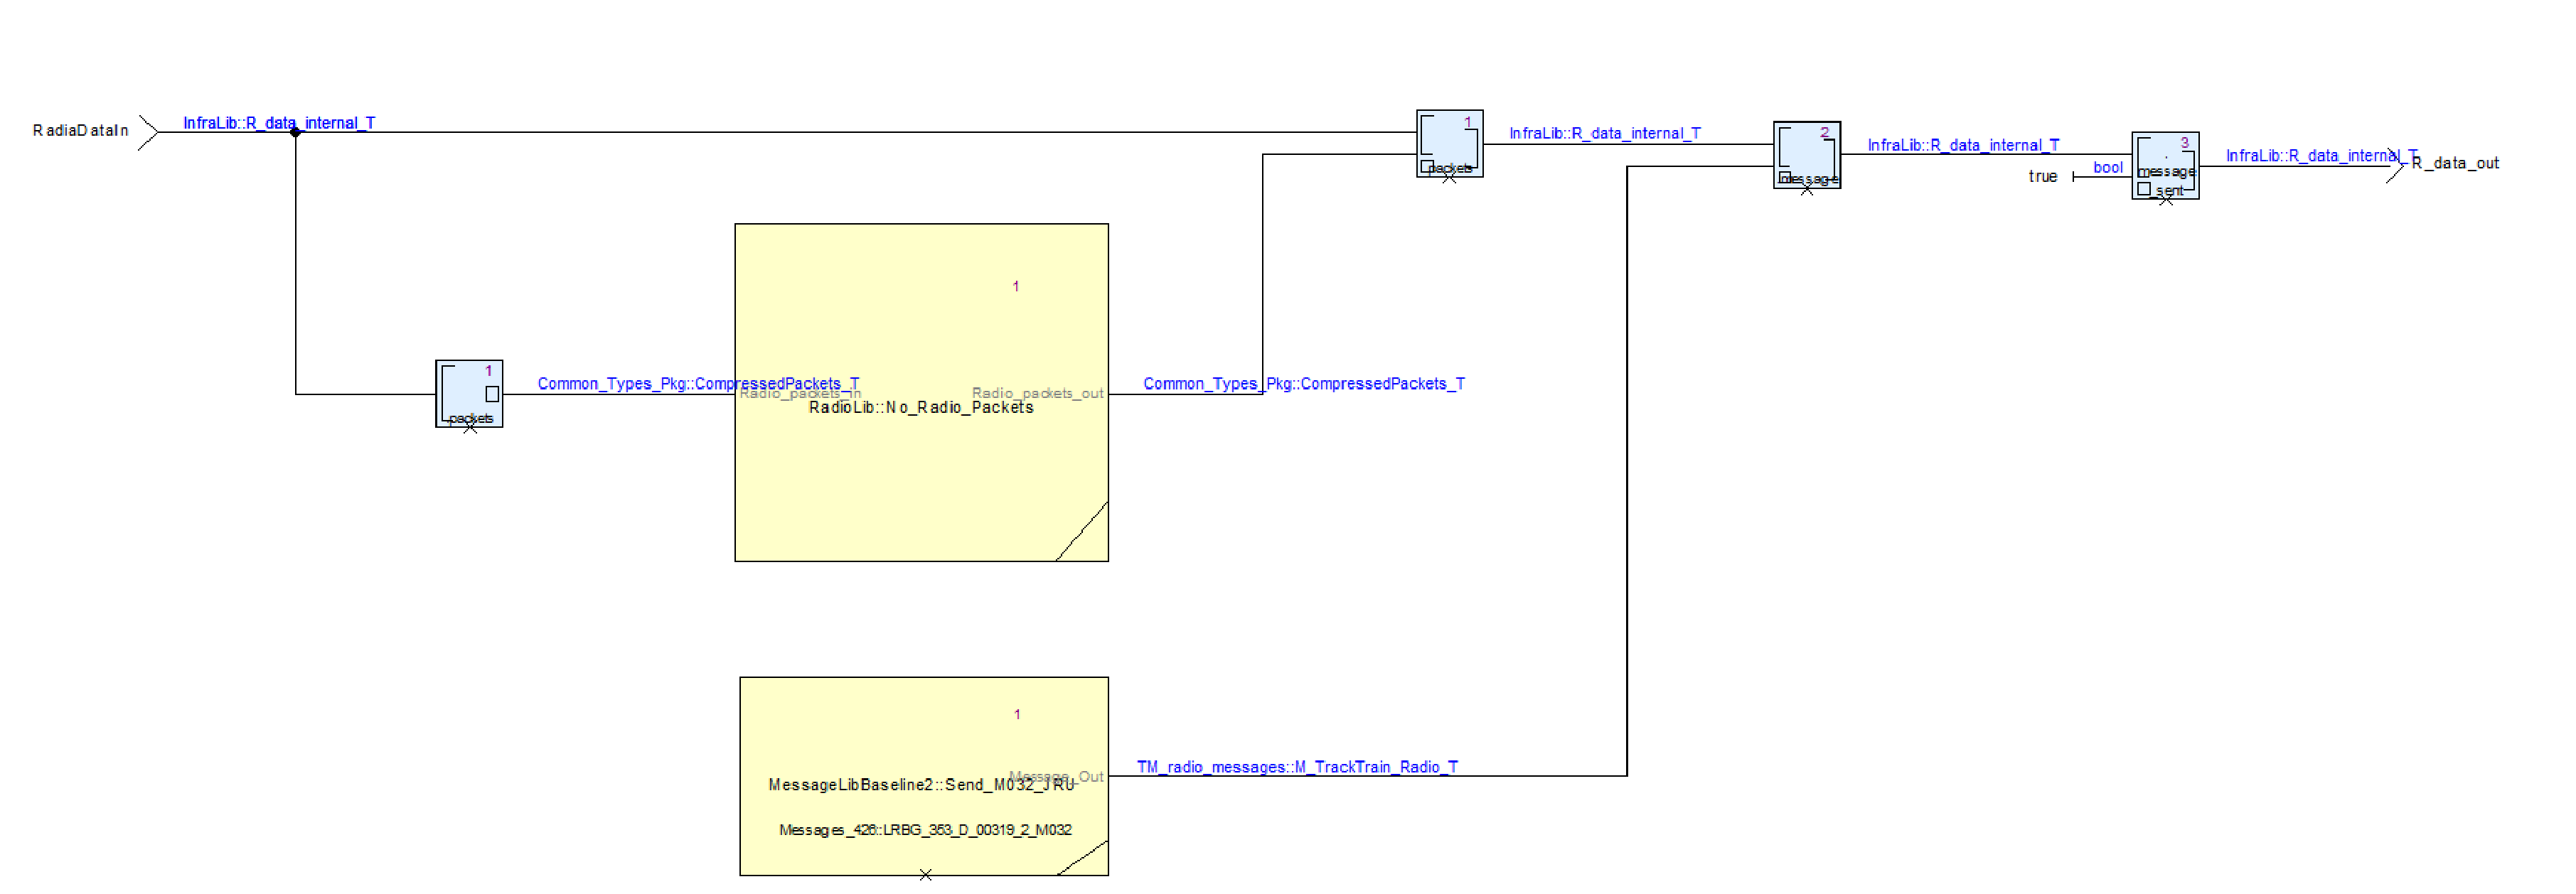
\includegraphics[width=6.5in]{images/composeRM.eps}
   \caption{Merge message information into the message/ packets stream (view from SCADE model)}
  \label{fig:composeRM}
\end{figure}
The operator \emph{RadioLib::No\_Radio\_Packets} simply passes along the packet stream without adding any information. \newline

If we look at a different message (Message 3, L2/3 Movement Authority), we explore the operator SendRadioPackets\_LRBG\_351\_D\_00054\_9\_M003, which plugs in the same place as our RadioLib::No\_Radio\_Packets. This operator merges a set of packets into the packet stream. We can see that the pattern is identical to sending packets from a balise. Even the data structures are the same (see figure \ref{fig:m3})

\begin{figure}[H]
  \centering
  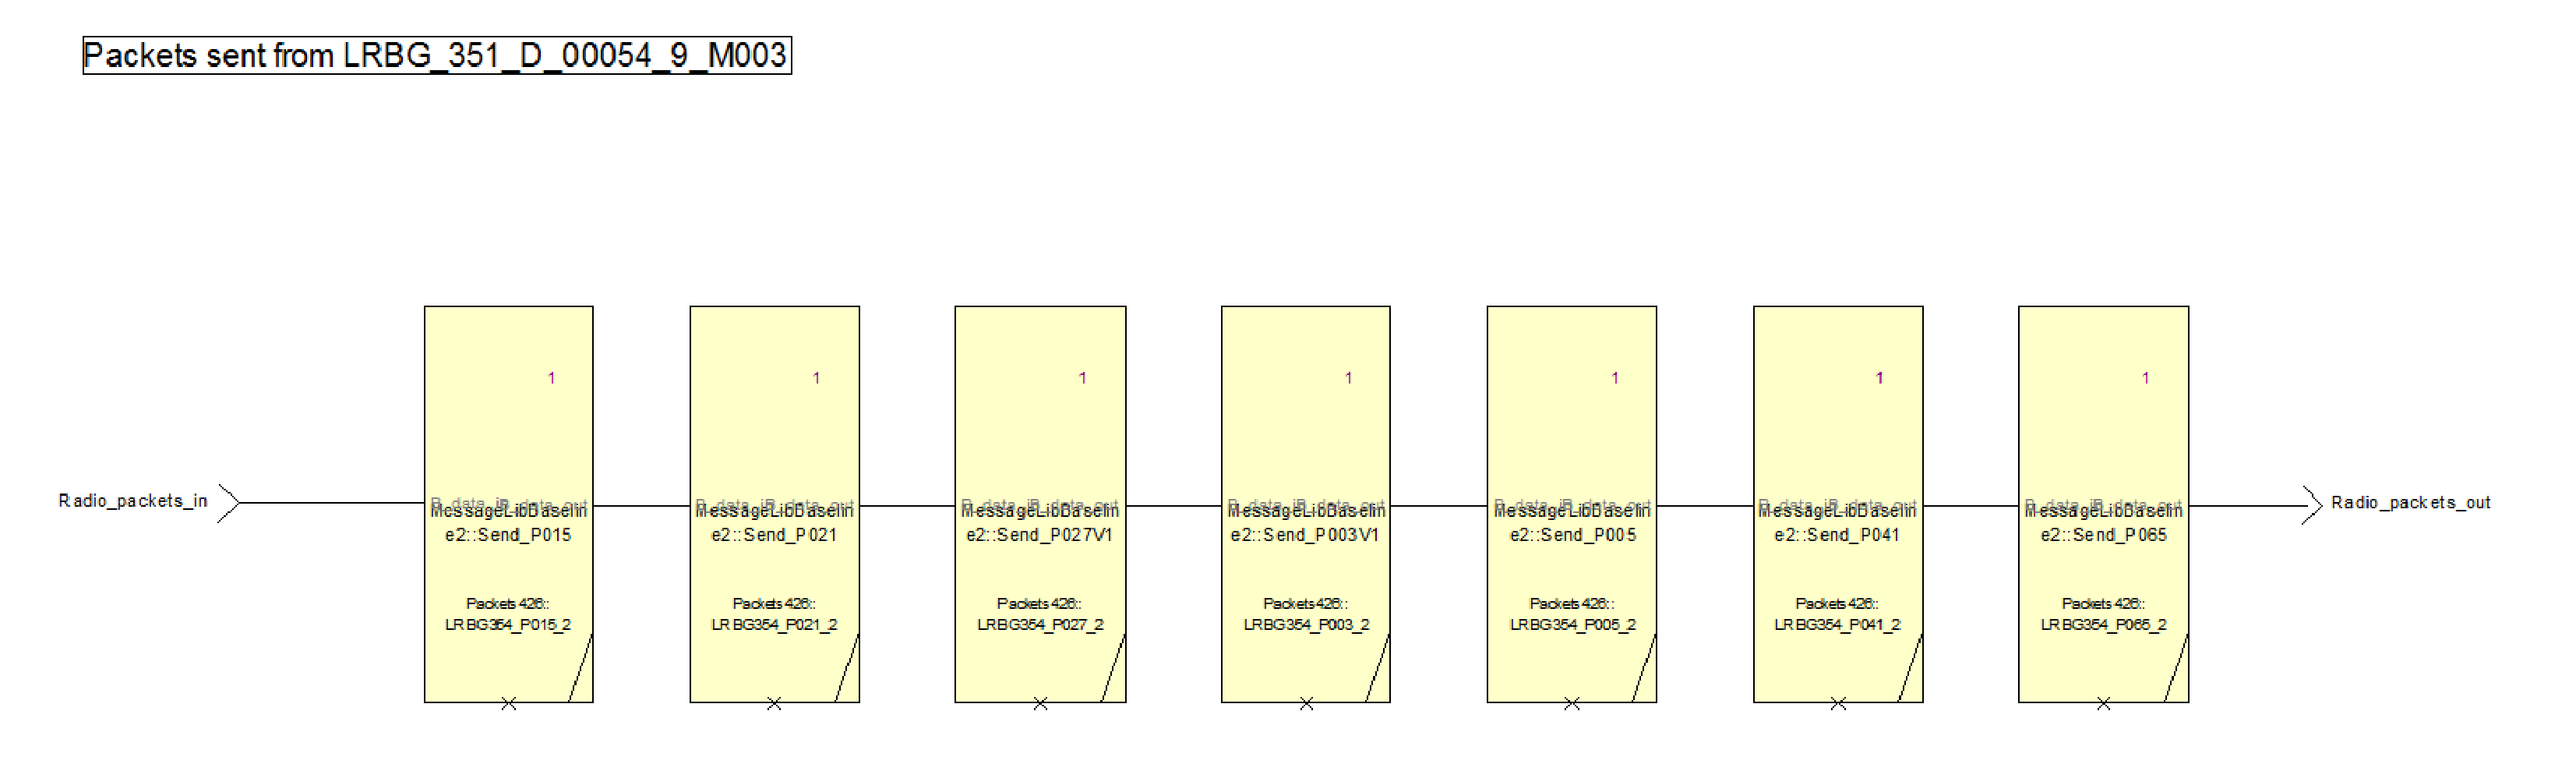
\includegraphics[width=6.5in]{images/RM3.eps}
   \caption{Composing packets for a L2/3 Movement Authority message (view from SCADE model)}
  \label{fig:m3}
\end{figure}


\section{Implementation of additional user stories}

During the remaining period of openETCS, we may extend the track model to reflect additional scenarios.
We consider the balise part of the model as stable, as we are on a Level 2 infrastructure.\newline
Hence, we simply need to add or derive radio message models consisting of specific combinations of
\begin{itemize}
 \item Messages and Packets
 \item Trigger conditions
\end{itemize}

\subsection{Building your own tracks}

A detailed HOWTO guide on how to build new test tracks using the provided design templates and libraries will be provided for the final iteration of openETCS.

\section{Connecting with existing environments}

The dynamic track model is intended to be used as part of the existing testing and validation ecosystem around ETCS.
It could also be extended, using the same principles, to reflect national systems, or be used for experiments with new approaches such as ERTMS Regional. 

\subsection{Subset-076}

The Dynamic Track Simulation model relies on a formalisation of Subset-026 chapters 6,7, and 8 provided by the openETCS TrackMessages library. This library provides data structures which are compatible with Subset-076, but require some interfacing work. openETCS WP4 is working on the integration.

\subsection{Subset-094}

Thanks to the open architecture of openETCS and the openETCS track simulation approach, integration with existing Subset-094 compliant onboard testing systems is feasible. 
Extension of the openETCS demonstrator to a full Subset-094 implementation may be an interesting topic for future exploitation of the project's results. 

\section{Closing remarks}

We have extended the openETCS approach to exploring the possibilities of formal modelling also on Trackside ETCS infrastructure. The main focus for this iteration was on creating an extensible, modular approach to reflect the dynamic behaviour of trackside train automation installations.\newline
We had, to a large extent, to rely on reverse engineering techniques and are aware that the model is far from complete as far as the RBC messages are concerned. 


%-------------------examples below



\nocite{*}

\bibliographystyle{unsrt}
\bibliography{erdc}



\begin{thebibliography}{9}

\bibitem{CCS-TSI}
  European Rail Agency:
  \emph{Applicable standards in HS Control-Command and Signalling TSI (2006/860/EC)}
  ERA/Interoperability/JCP/hpi/2008/208 Version 1.0, 2008
\bibitem{SRS026-6}
  ERA - UNISIG - EEIG ERTMS USERS GROUP Subset-026 
  \emph{System Requirements Specification Chapter 6 Management of older System Versions Issue 3.3.0}.
 2012.
\bibitem{SRS026-7}
  ERA - UNISIG - EEIG ERTMS USERS GROUP Subset-026
  \emph{System Requirements Specification Chapter 7 ERTMS/ETCS language Issue 3.3.0}.
 2012.
 \bibitem{SRS026-8}
  ERA - UNISIG - EEIG ERTMS USERS GROUP Subset-026
  \emph{System Requirements Specification Chapter 8 Messages Issue 3.3.0}.
 2012.
\bibitem{Subset076}
  ERTMS/ETCS Subset-076
  \emph{Test cases, Version 3.1.0}.
 2015.
\bibitem{Subset094}
  ERTMS/ETCS Subset-094:
  \emph{FUNCTIONAL REQUIREMENTS FOR AN ON-BOARD REFERENCE TEST FACILITY, Version 3.0.0}.
 2014.
\bibitem{muttram08}
  Rod Muttram, Bombardier:
  \emph{Delivering the upgraded Amsterdam-Utrecht corridor.}.
  HighSpeed 2008 Amsterdam 6th World Congress on High Speed Rail,
  2008.
\bibitem{uic08}
  Paolo De Cicco, Olivier Lev\^eque, UIC:
  \emph{ETCS Implementation Handbook}.
  Paris, 2008.
  \bibitem{OpRules}
  ProRail:
  \emph{Het rijden van ETCS treinen op het trace Amsterdam-Utrecht}.
  Version 7.0, 2010, German Translation by Shivana Daparoe
    \bibitem{Esterel50128}
  Esterel Technologies:
  \emph{Methodology Handbook: 
Efficient Development of Safe Railway Applications Software with EN 50128 Objectives Using SCADE Suite\textregistered}.
  Third Edition (Revision 1), Elancourt, 2012
    \bibitem{Alstom-oETCS}
  S. Besure:
  \emph{Alstom OpenETCS WP3 contribution:
EXTRACT FROM ALSTOM TRB MODEL}.
  OpenETCS\_DNOT\_0001 Rel. A, Charleroi 2013
\end{thebibliography}

%===================================================
%Do NOT change anything below this line

\end{document}
